\documentclass{beamer}

\usepackage{beamerthemesplit}

\usepackage{xmpmulti}
\usepackage{animate}
\usepackage{amsmath}
\usepackage{physics}
\usepackage{xcolor}
\usepackage{graphicx}
\usepackage{fontawesome5}
\usepackage{tcolorbox}

\usepackage{amssymb}
\usepackage{multirow}
\usepackage{mathtools}

\usepackage{physics}
\usepackage{mathrsfs}

\usepackage{tikz}
\usetikzlibrary{calc}

\usetheme{Copenhagen}
\useoutertheme{infolines}

\newcommand{\iu}{{i\mkern1mu}}

\title[Systematic Description of W.M.]{A Systematic Description of the Wobbling Motion in Odd-Mass Nuclei Within a Semi-Classical Formalism}


% old author setup
% \author[Robert Poenaru]{%
%     \parbox[t]{0.5\textwidth}{%
%         \textbf{Author} \\
%         Robert Poenaru\inst{1} \inst{2}
%     }%
%     \parbox[t]{0.5\textwidth}{%
%         \textbf{Scientific Coordinator} \\
%         Prof. Em. Dr. A. A. Raduta\inst{2}
%     }%
% }
% \institute[DFT]{
% \inst{1} Doctoral School of Physics, UB \and %
% \inst{2} Department of Theoretical Physics, IFIN-HH
% }

% manual override for a side-by-side author view
\author[Robert Poenaru]{%
    \parbox[t]{0.45\textwidth}{%
		\centering
		\textbf{PhD Candidate} \\
		Robert Poenaru\texorpdfstring{$^{1,2}$}{(1,2)}
    }%
    \parbox[t]{0.45\textwidth}{%
		\centering
        \textbf{Scientific Supervisor} \\
        Prof. Dr. Em. A. A. Raduta\texorpdfstring{$^{2}$}{(2)}
    }%
}
\institute[IFIN-HH]{\texorpdfstring{$^{1}$}{1}Doctoral School of Physics, UB \\ \texorpdfstring{$^{2}$}{2}Department of Theoretical Physics, IFIN-HH}

\date[\today]{\textit{A presentation for the degree of Doctor of Philosophy}\vspace{0.2cm} \\ \today} % Presentation date or conference/meeting name, the optional parameter can contain a shortened version to appear on the bottom of every slide, while the required parameter value is output to the title slide

%%%%%%%%%%%%%%%%%%%%%%%%%%%%%%%%%%%%%
%%%%%%% start of the document %%%%%%%
%%%%%%%%%%%%%%%%%%%%%%%%%%%%%%%%%%%%%

\begin{document}

% trick to show a the first slide without the header
{\setbeamertemplate{headline}{}
\begin{frame}
	\titlepage % Output the title slide, automatically created using the text entered in the PRESENTATION INFORMATION block above
\end{frame}}


\AtBeginSection[]{
	\begin{frame}{Outline}
	\small \tableofcontents[currentsection, hideothersubsections]
	\end{frame} 
}

% \begin{frame}
%     \frametitle{TOC}
%     \tableofcontents
% \end{frame}

\section{Aim and Motivation}

\begin{frame}
    \frametitle{Aim}
    \begin{block}{\faClipboard\ Research Objectives}
        \begin{itemize}
            \item Extend the current interpretation of the \textbf{Nuclear Triaxiality} in the context of its unique fingerprint: \textbf{Wobbling Motion}. % {\footnotesize\emph{from a theoretical standpoint}}
            \item Adopt a framework that is as close as possible to a \textbf{classical picture}.
            % \item Provide new formalisms for the phenomena related to \textbf{nuclear deformation}.
        \end{itemize}
    \end{block}
    \begin{exampleblock}{\faClipboard\ Objectives exclusive to the thesis}
        \begin{itemize}
            \item Enough context towards a better understanding of the underlying concepts, methods, and results.
            \item \faGithub\ create a completely \emph{open-source} project.
        \end{itemize}
    \end{exampleblock}
\end{frame}

\begin{frame}
	\frametitle{Motivation}
    \vspace{-0.2cm}
    \begin{itemize}
        \item \textbf{Nuclear Triaxiality} recently became a \emph{hot topic} within the scientific community.
        \item Identifying nuclei with triaxial deformations represents a real \textbf{experimental} and \textbf{theoretical} challenge.
        % \item Experimental side: large setups, complex electronics, 
        % \item Theoretical side: cumbersome models, approximations, abstractions...
    \end{itemize}
    \vspace{-0.2cm}
    \begin{figure}
        \centering
        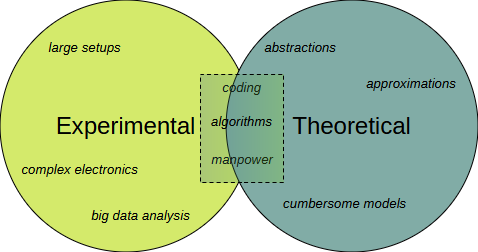
\includegraphics[width=0.85\textwidth]{figures/exp_vs_theory.png}
    \end{figure}
\end{frame}

\section{Nuclear Shapes}

\begin{frame}
	\frametitle{Nuclear Deformation}
	\begin{exampleblock}{Nuclear shapes}
		Most generally described in terms of the \textbf{nuclear radius}:
		\begin{align}
			R(\theta,\varphi)=R_0\left(1+\sum_{\lambda=0}^{^\infty}\sum_{\mu=-\lambda}^\lambda\alpha_{\lambda\mu}Y_\lambda^\mu(\theta,\varphi)\right)\nonumber
		\end{align}
	\end{exampleblock}
	% \begin{itemize}
	% 	\item The $\alpha_{\lambda\mu}$ are collective coordinates $\Longrightarrow$ \emph{vibrations of the nucleus}.
	% 	\item $Y_\lambda^\mu$ are the spherical harmonics.
	% \end{itemize}
	\begin{block}{Quadrupole deformations $\lambda=2$}

		\begin{itemize}
			\item {\color{red}For us:} Most relevant modes are the \textbf{quadrupole vibrations} $\lambda=2$ $\Longrightarrow$ \emph{Play a crucial role in the rotational spectra of nuclei:}
			\item $\alpha_{2\mu}$ reduced to only two \emph{deformation parameters}: $\beta_2$ (\textbf{eccentricity}) and $\gamma$ (\textbf{triaxiality}) (\textit{Bohr and Mottelson, 1969}).
		\end{itemize}
		% \begin{align}
		% 	R(\theta,\varphi)=R_0\left(1+\sum_{\mu=-2}^2\alpha_{2\mu}Y_2^\mu(\theta,\varphi)\right)\ ,
		% \end{align}
	\end{block}
\end{frame}

\begin{frame}
	\frametitle{Axial shapes}
	\vspace{-0.2cm}
	\begin{itemize}
		\item Most of the nuclei are either \textbf{spherical} or \textbf{axially symmetric} in their ground-state \textit{(Budaca, 2018)}.
		\item Moments of inertia: $\mathcal{I}_{1,2,3}$: two are equal, one is different.
	\end{itemize}
	\vspace{-0.4cm}
	\begin{figure}
		\centering
		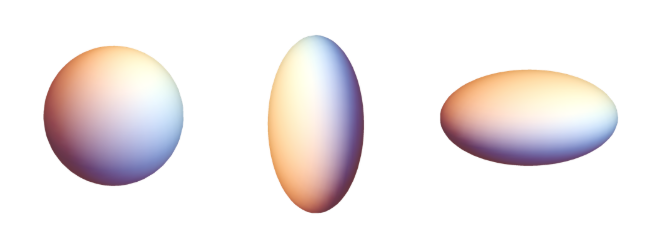
\includegraphics[scale=0.38]{figures/nuclear_shapes.png}
		\caption{\textbf{spherical:} $\beta_2=0$\ \textbf{prolate:} $\beta_2>0$\ \textbf{oblate:} $\beta_2<0$.\ ($\gamma=0^\circ$).}
	\end{figure}
\end{frame}

\begin{frame}
	\frametitle{Non-axial shapes}
	\vspace{-0.2cm}
	\begin{itemize}
		\item The triaxiality parameter $\gamma\neq 0^\circ$: departure from axial symmetry.
		\item Moments of inertia: $\mathcal{I}_{1}\neq\mathcal{I}_{2}\neq\mathcal{I}_{3}$.
	\end{itemize}
	\vspace{-0.2cm}
	\begin{figure}
		\centering
		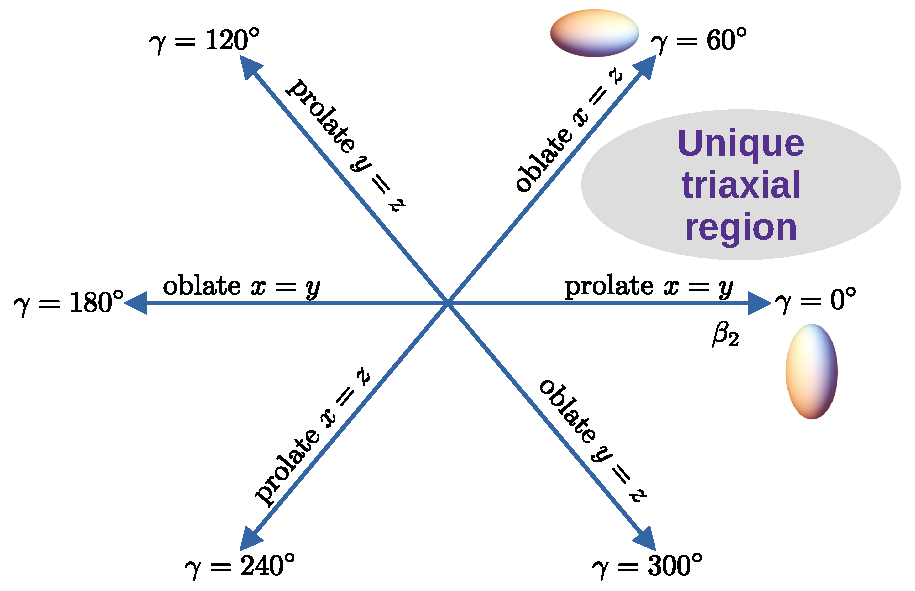
\includegraphics[scale=0.49]{figures/nice_diagram.pdf}
		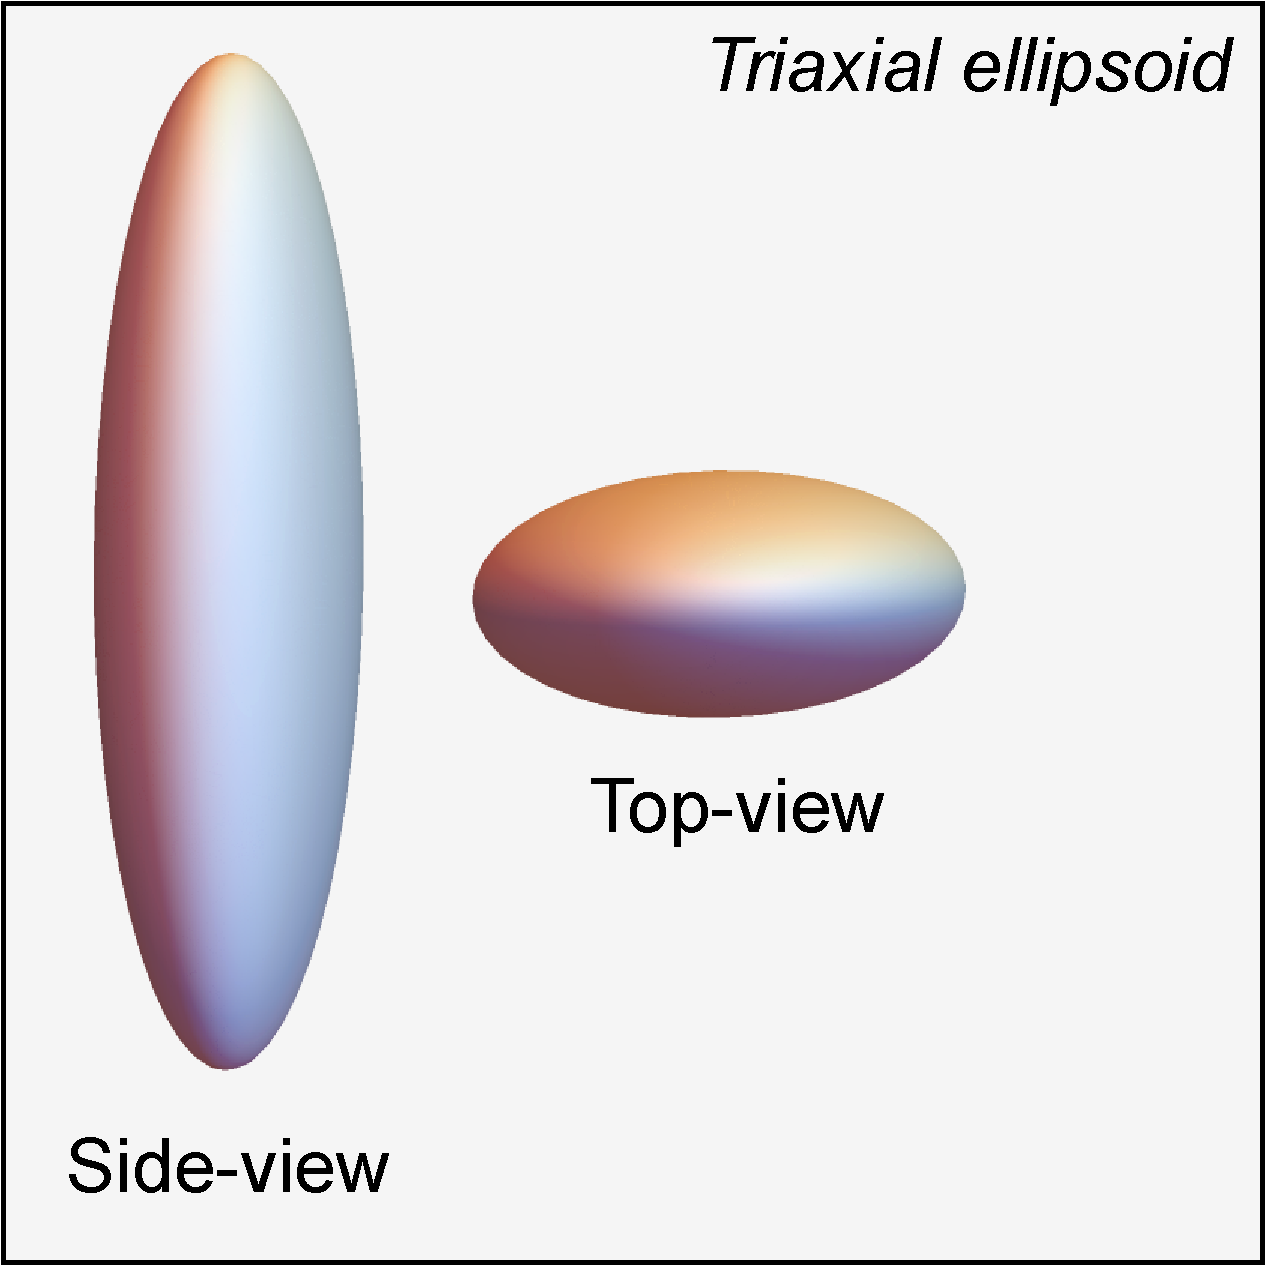
\includegraphics[scale=0.20]{figures/triaxial-shape.pdf}
		\vspace{-0.41cm}
	\end{figure}
\end{frame}

\section{Triaxiality and Wobbling Motion}

\begin{frame}
	\frametitle{Fingerprints of Triaxiality}
	\begin{block}{Evidence \faSearch}
		\begin{itemize}
			\item Currently, there are \textbf{only two} well-established phenomena uniquely attributed to triaxial deformation.
			\begin{enumerate}
				\item \textbf{Wobbling Motion} - WM (\emph{Bohr and Mottelson, 1970s})
				\item Chiral Motion - $\chi$M (\emph{Frauendorf, 1997})
			\end{enumerate}
			\item These two can be measured/detected experimentally.
		\end{itemize}
	\end{block}
	\begin{exampleblock}{\textbf{Goal} \faClipboard}
		\textbf{Describe the elusive character of Wobbling Motion in the context of nuclear triaxiality.}
	\end{exampleblock}
\end{frame}

\begin{frame}
	\frametitle{\faSearch\ Probing triaxiality in nuclei}
    Triaxial nuclei can be observed/obtained in several experiments:
    \begin{itemize}
        \item Nuclear fission: $A\ \rightarrow\ B\ +\ C$
        \item Nuclear fusion: $X\ +\ Y\ \rightarrow\ Z$
        \item \textbf{Fusion-evaporation reactions}: {\color{red}Long-lived} + {\color{red}enhanced deformation}
        \vspace{-0.3cm}
        \begin{align}
            {\color{blue}Beam(N_1,E)}\ +\ {\color{magenta}Target(N_2)}\longrightarrow N_3^*\rightarrow\dots\rightarrow {\color{purple}triaxial(N_4)} \nonumber
        \end{align}
    \end{itemize}
	\vspace{-0.3cm}
    \begin{figure}
        \centering
        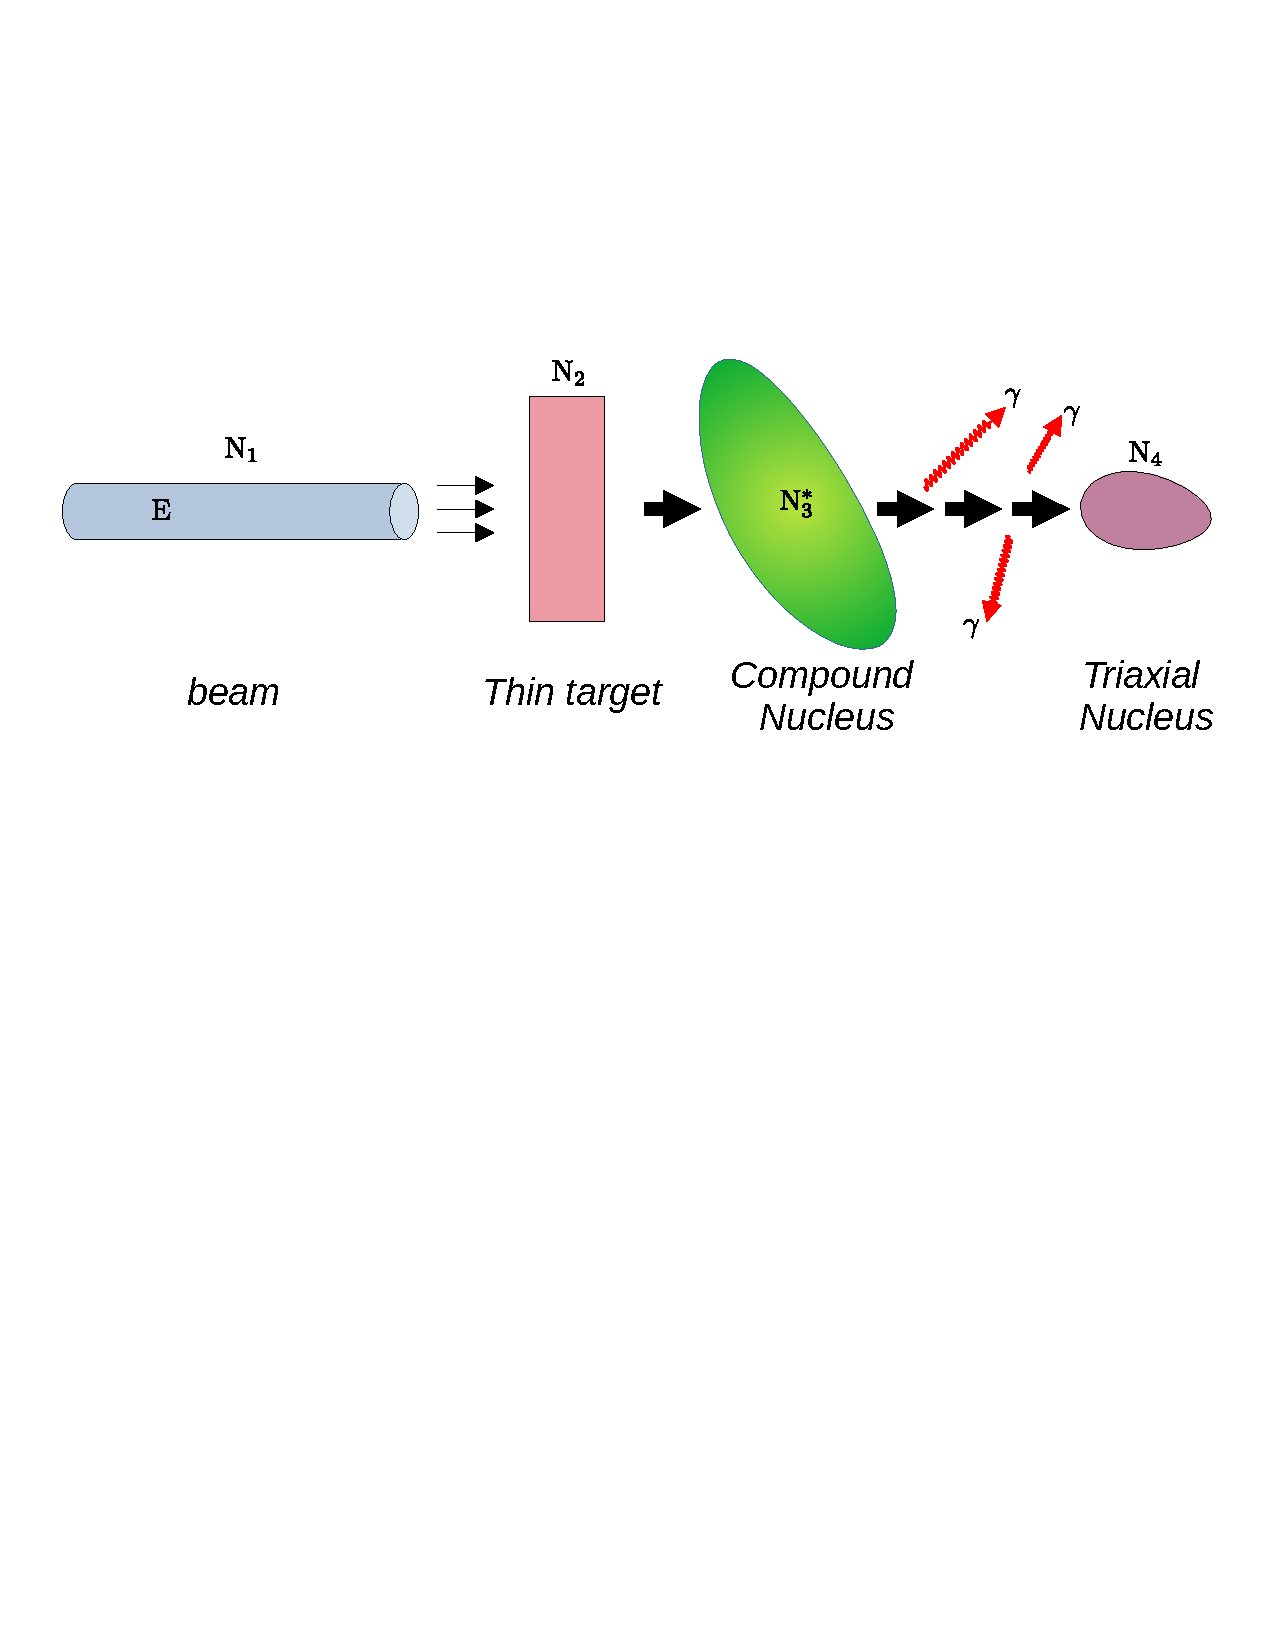
\includegraphics[width=0.99\textwidth]{figures/fusion-evaporation.pdf}
    \end{figure}
\end{frame}

\begin{frame}
	\frametitle{\faSearch\ Nuclear facilities}
	\vspace{-0.3cm}
	\begin{columns}
		\column{0.4\textwidth}
		\begin{figure}
		\centering
		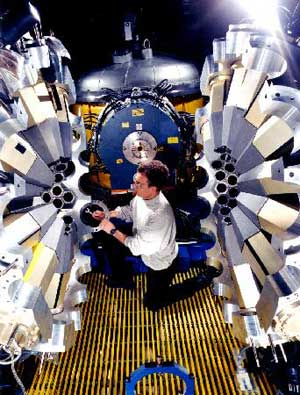
\includegraphics[width=0.88\textwidth]{figures/gsfig.jpg}
		\caption{Gammasphere detector, ANL-ATLAS USA. \textit{Source: aps.org}}
	\end{figure}
	\column{0.6\textwidth}
	\begin{figure}
		\centering
		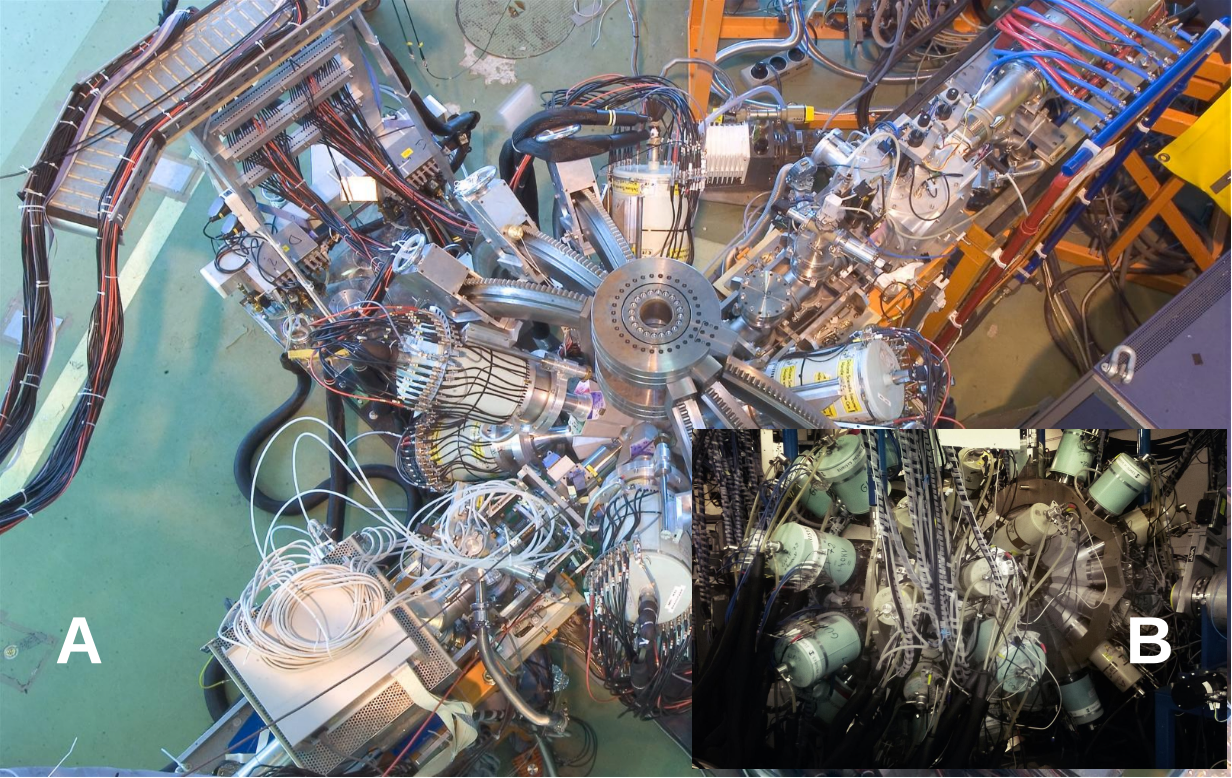
\includegraphics[width=0.99\textwidth]{figures/isolde_cern_2.png}
		\caption{a) IDS detector, CERN. \textit{Source: isolde.web.cern.ch} b) JUROGAM II, Finland. \textit{Source: twitter.com}}
		\end{figure}
	\end{columns}
\end{frame}

\begin{frame}
	\frametitle{\faSearch\ High-Spin Physics @ IFIN-HH}
		\begin{figure}
		\centering
		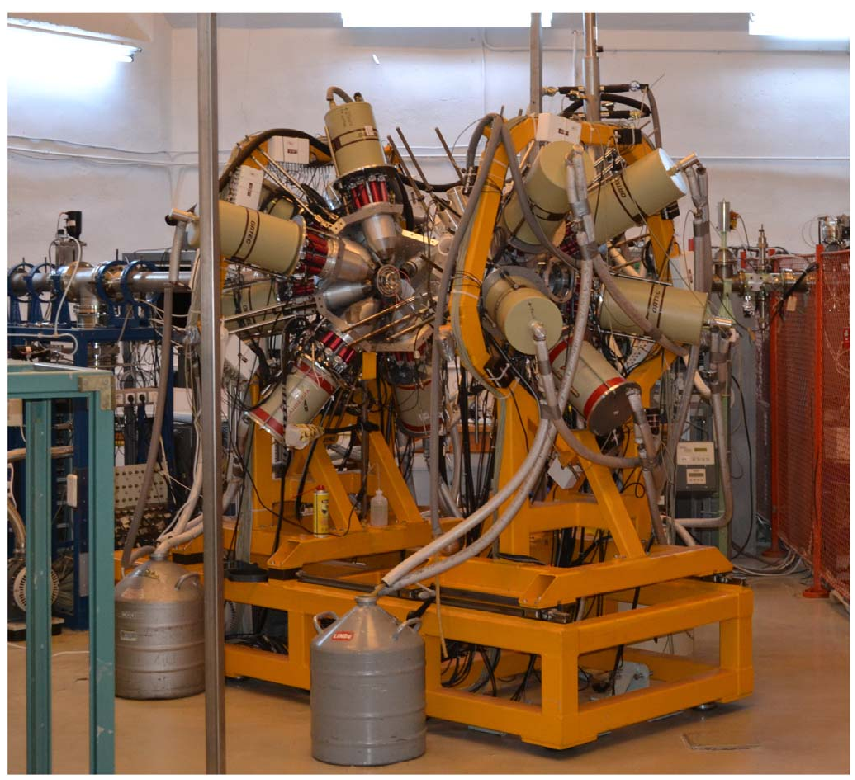
\includegraphics[scale=0.31]{figures/ro-sphere.pdf}
		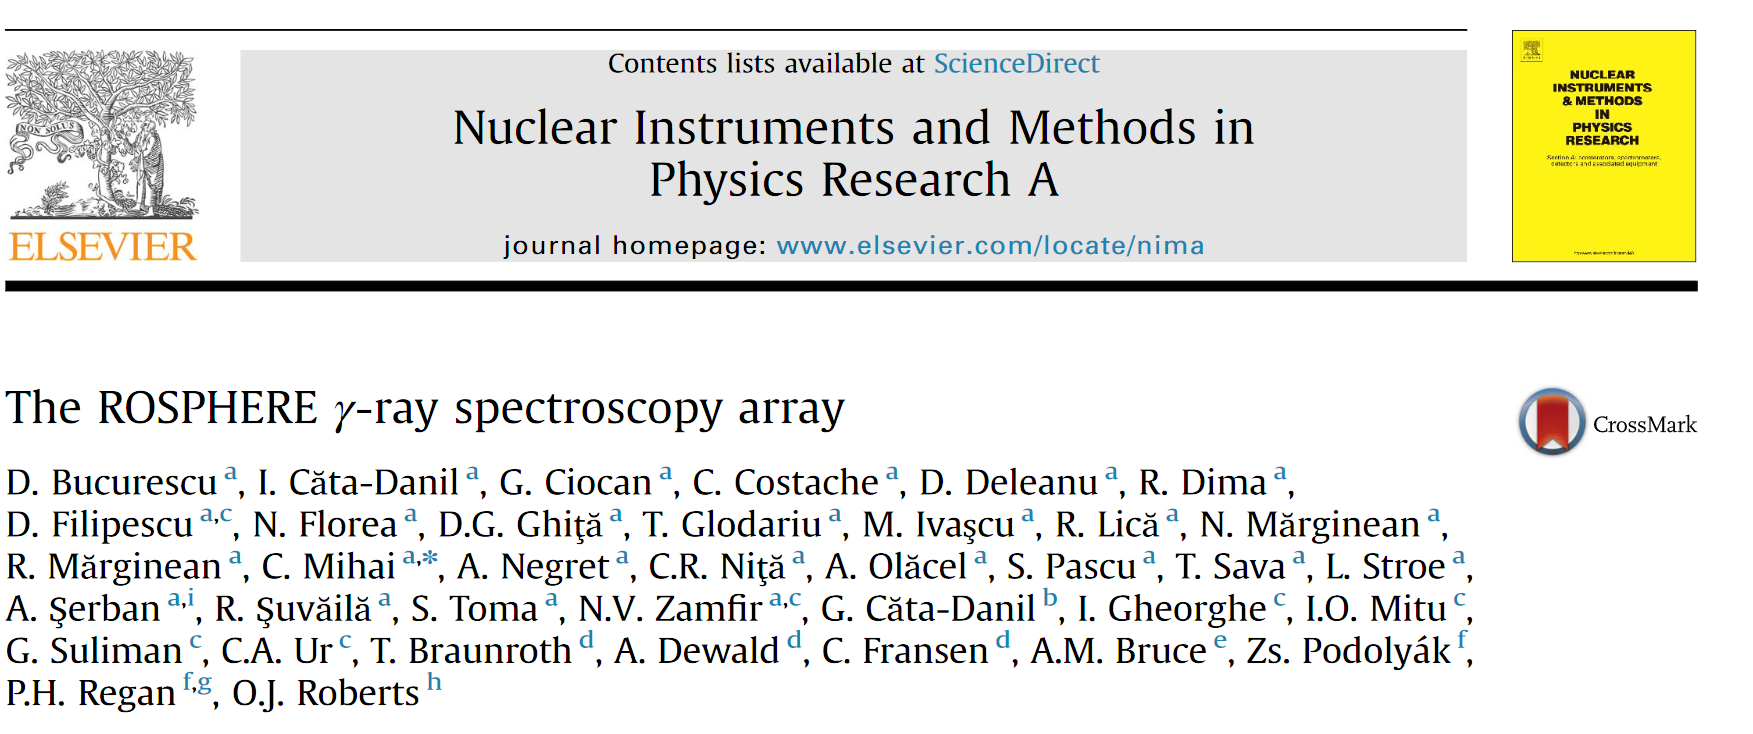
\includegraphics[scale=0.15]{figures/rosphere-paper.png}
		\caption{ROSPHERE, IFIN-HH. \textit{Source: tandem.nipne.ro}}
	\end{figure}
\end{frame}

\begin{frame}
	\frametitle{Wobbling Motion}
	\vspace{-0.4cm}
	\begin{columns}
		\begin{column}{0.55\textwidth}
			\begin{center}
				\begin{tikzpicture}[node distance=1.5cm]
					\node[draw, fill=blue!20!white, text width=3cm, text centered, minimum height=1cm] (box1) {$\gamma\neq0^\circ$};
					\node[draw, fill=blue!20!white, text width=4cm, text centered, minimum height=1cm, below of=box1] (box2) {MOI anisotropy};
					\node[draw, fill=blue!20!white, text width=6cm, text centered, minimum height=1cm, below of=box2] (box3) {\emph{main rotation} around $\mathcal{J}_\text{max}$ is disturbed by the other two axes};
					\draw[->] (box1) -- (box2);
					\draw[->] (box2) -- (box3);
				\end{tikzpicture}
			\end{center}
		\end{column}
		\begin{column}{0.45\textwidth}
			\begin{figure}
				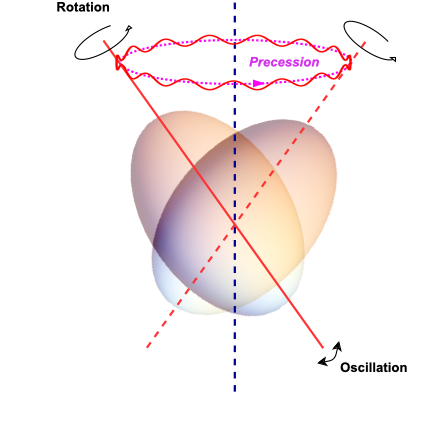
\includegraphics[width=\textwidth]{figures/wobbling-schematic.png}
			\end{figure}
		\end{column}
	\end{columns}
	\vspace{-0.4cm}
	\begin{alertblock}{Wobbling Effect}
		\begin{itemize}
			\item The \textbf{total angular momentum} of the nucleus \textbf{precesses} and \textbf{oscillates} around $\mathcal{J}_\text{max}$.
		\end{itemize}
	\end{alertblock}
\end{frame}

\begin{frame}
	\frametitle{Wobbling Motion}
	\begin{exampleblock}{Harmonic oscillation}
		\begin{itemize}
			\item Precession of $\mathbf{I}$ is affected by \textbf{rotational frequency} and/or \textbf{tilting}
			\item Tilting only by "specific" amount $\rightarrow$ \textbf{harmonic character} $\rightarrow$ \textbf{wobbling phonon}: $n_w=0,1,2,\dots$.
		\end{itemize}
	\end{exampleblock}
	\begin{figure}
		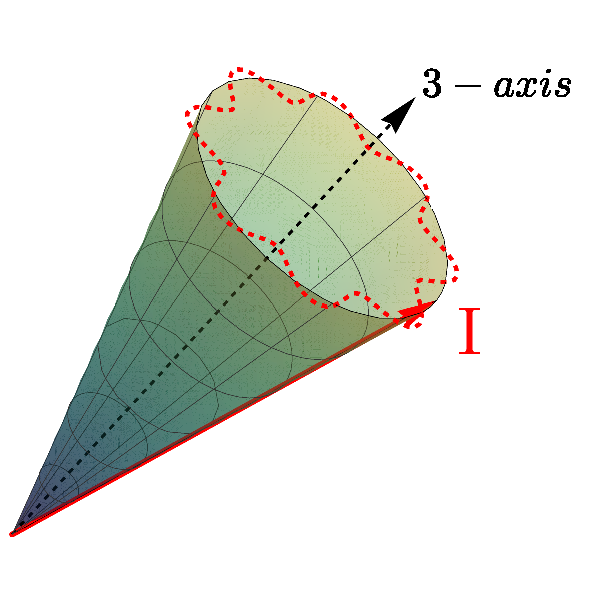
\includegraphics[width=0.32\textwidth]{figures/precessional_cone_2.pdf}
		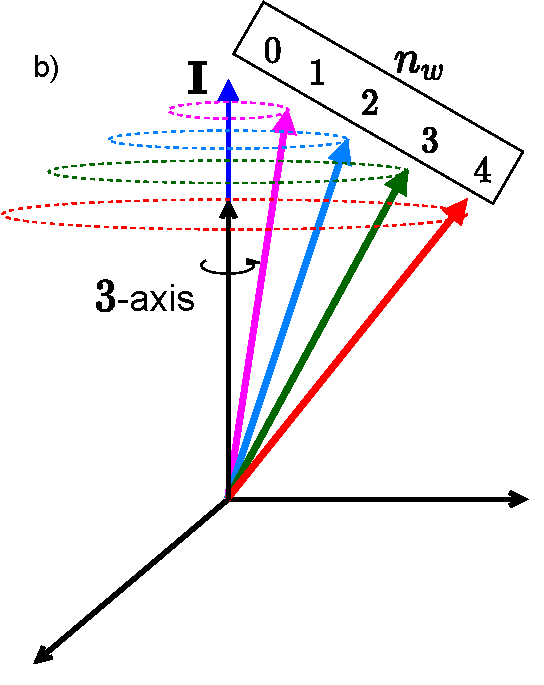
\includegraphics[width=0.3\textwidth]{figures/wobbling_n_schematic-2.pdf}
		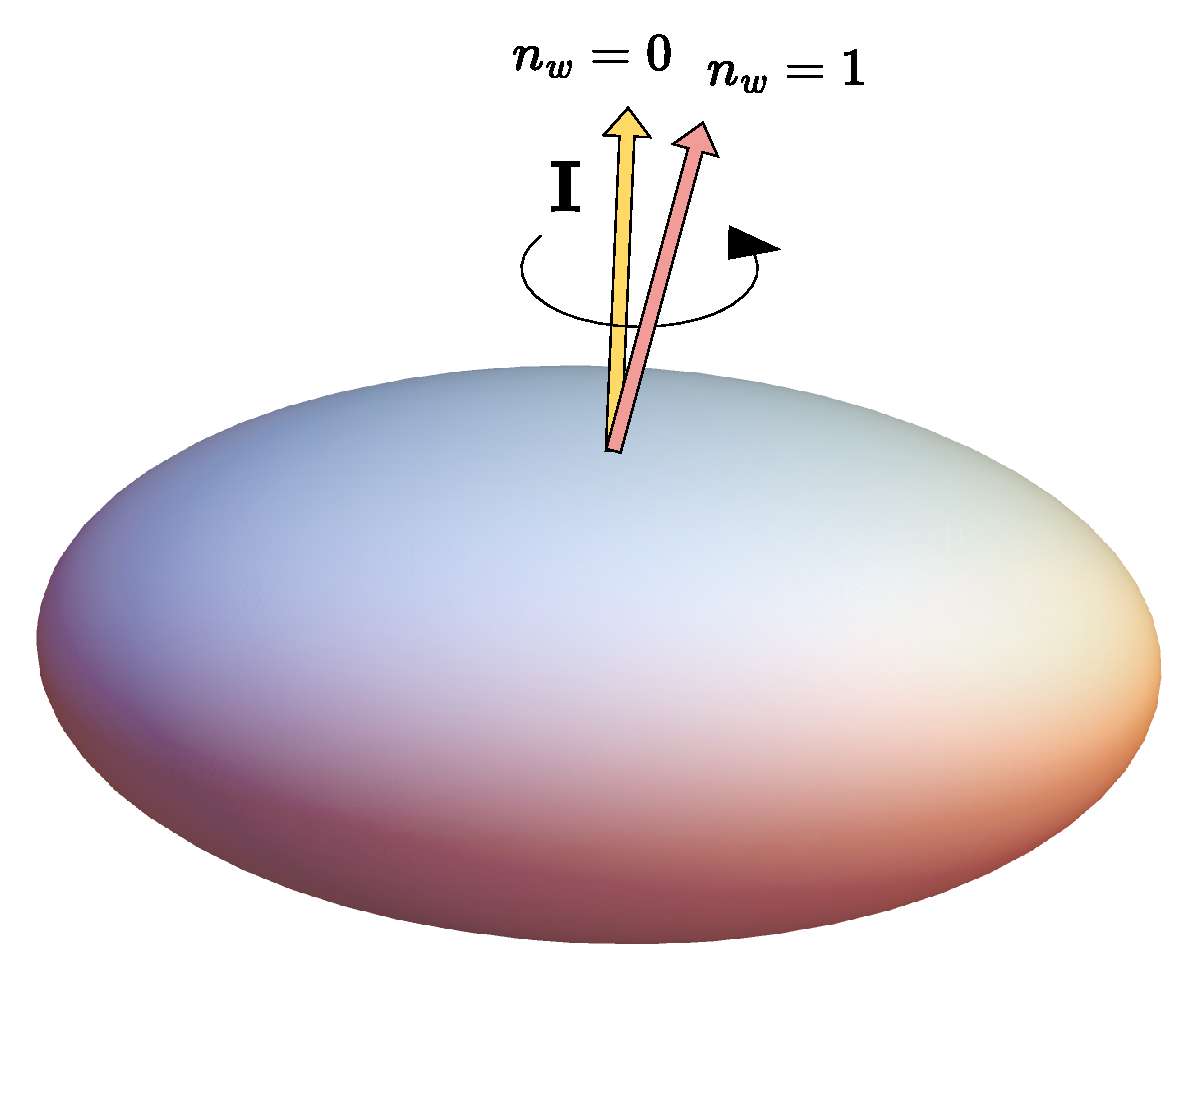
\includegraphics[width=0.34\textwidth]{figures/triaxial-shapes-even-A.pdf}
	\end{figure}
\end{frame}

\begin{frame}
	\frametitle{Wobbling Motion II}
	\vspace{-0.4cm}
	\begin{columns}
		\begin{column}{0.6\textwidth}
			\begin{figure}
				\centering
				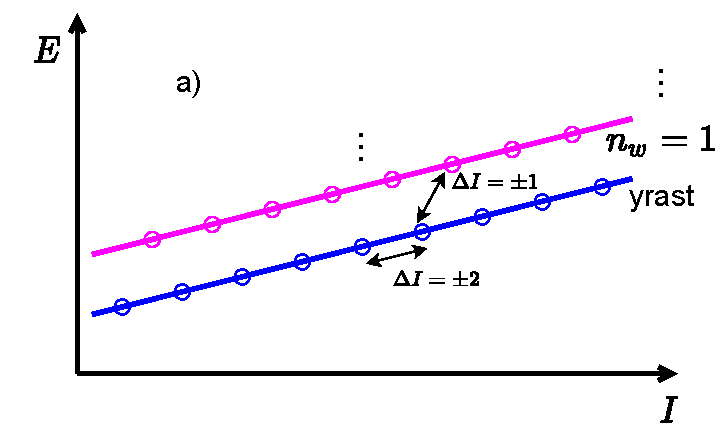
\includegraphics[scale=0.45]{figures/wobbling_n_schematic-1.pdf}
				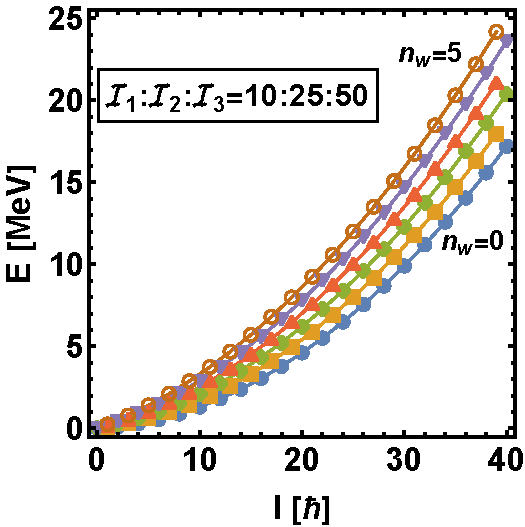
\includegraphics[scale=0.48]{figures/wobblingFreq-evenA.pdf}
			\end{figure}
		\end{column}
		\begin{column}{0.4\textwidth}
			\begin{figure}
				\centering
				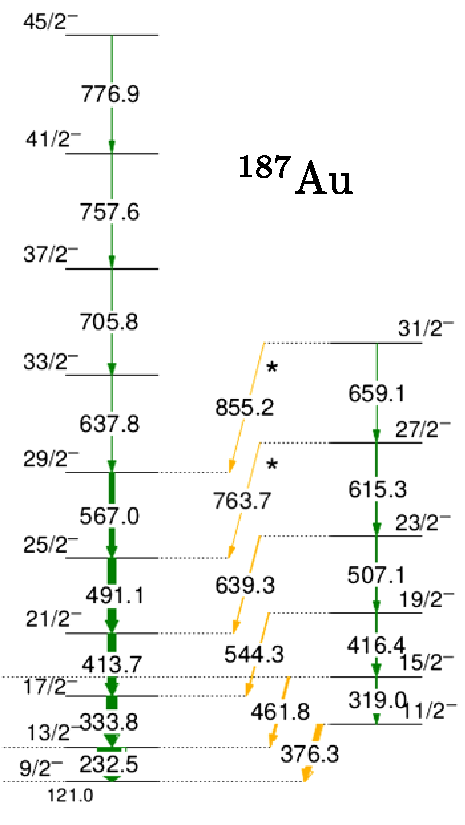
\includegraphics[width=0.8\textwidth]{figures/au_187_spectra.pdf}
			\end{figure}
			\vspace{-0.4cm}
			\textit{Sensharma, 2020}.
		\end{column}
	\end{columns}
\end{frame}

% \begin{frame}
%     \transduration<0-5>{0}
%     \multiinclude[<+->][format=png, graphics={width=\textwidth}]{figures/wobbler-gif/wobbler}
%     % \animategraphics[loop,controls,width=\linewidth]{10}{figures/wobbler-gif/wobbler-}{0}{5}
% \end{frame}

\begin{frame}
	\frametitle{Even-$A$ vs. Odd-$A$ Picture}
	\begin{itemize}
		\item Predicted for even-$A$ nuclei more than 50 years ago.
		\item First experimental evidence: $^{163}$Lu (\textit{Ødegård, 2001}). %  for \textbf{nuclear wobbling motion}
		\item Current mass-regions for wobblers: $A\approx[130,160,180]$.
	\end{itemize}
	\begin{figure}
		\centering
		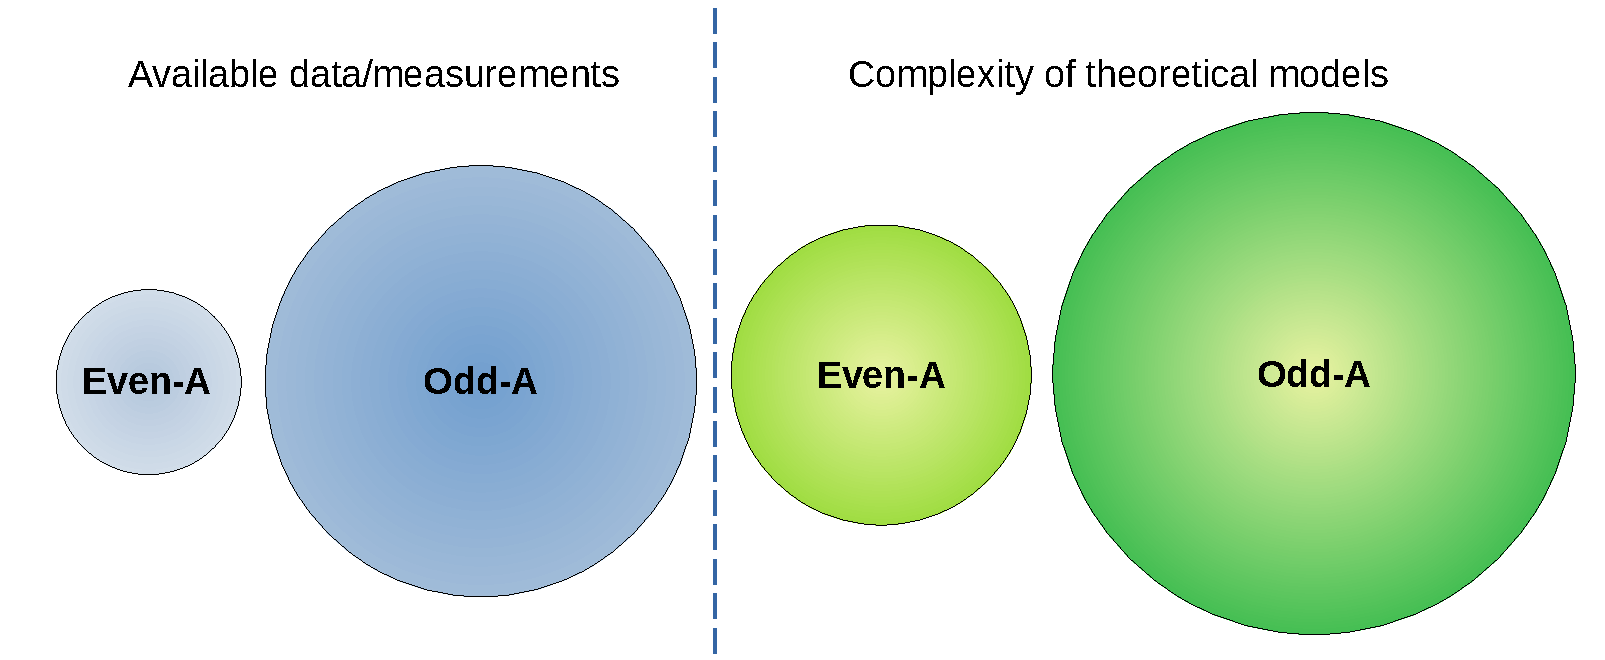
\includegraphics[width=0.99\textwidth]{figures/even-vs-odda.pdf}
	\end{figure}
\end{frame}

% \begin{frame}
% 	\frametitle{Wobblers in the A=130 mass region}
% 	\begin{figure}
% 		\centering
% 		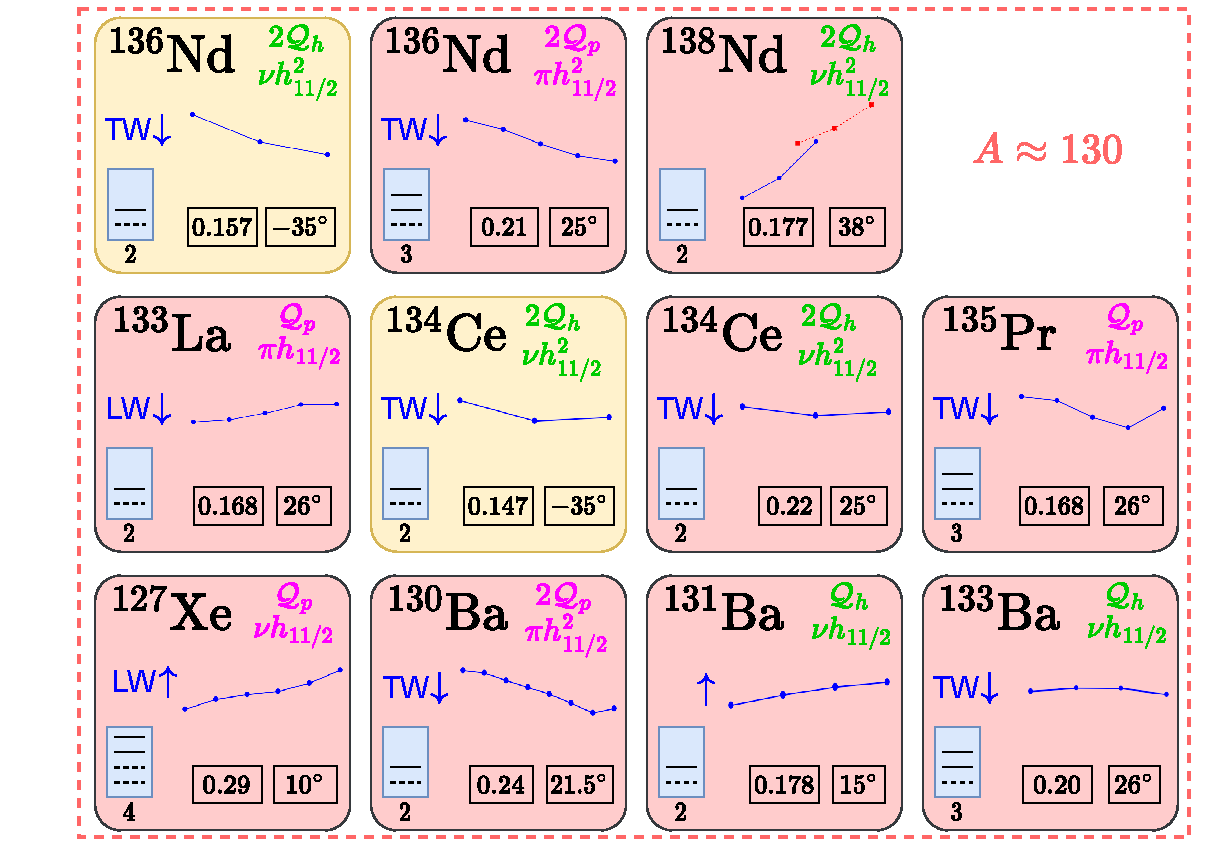
\includegraphics[width=0.87\textwidth]{figures/wobblers-chart-2.pdf}
% 	\end{figure}
% \end{frame}

% \begin{frame}
% 	\frametitle{Wobblers in the A=160 mass region}
% 	\begin{figure}
% 		\centering
% 		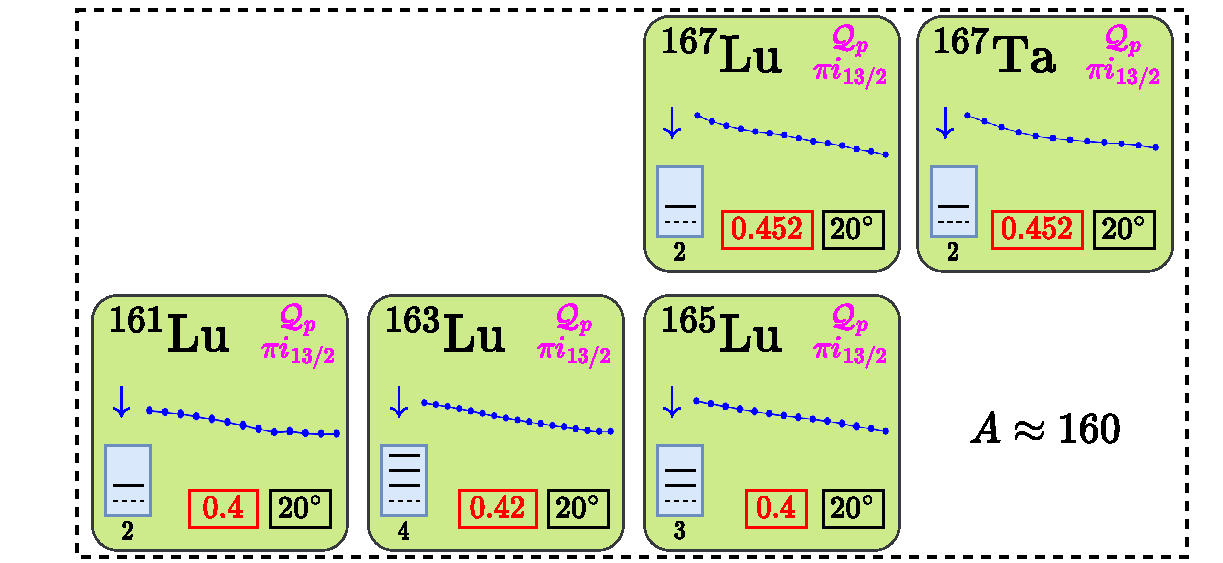
\includegraphics[width=0.99\textwidth]{figures/wobblers-chart-4.pdf}
% 	\end{figure}
% \end{frame}

% \begin{frame}
% 	\frametitle{Wobblers in the A=180 mass region}
% 	\begin{figure}
% 		\centering
% 		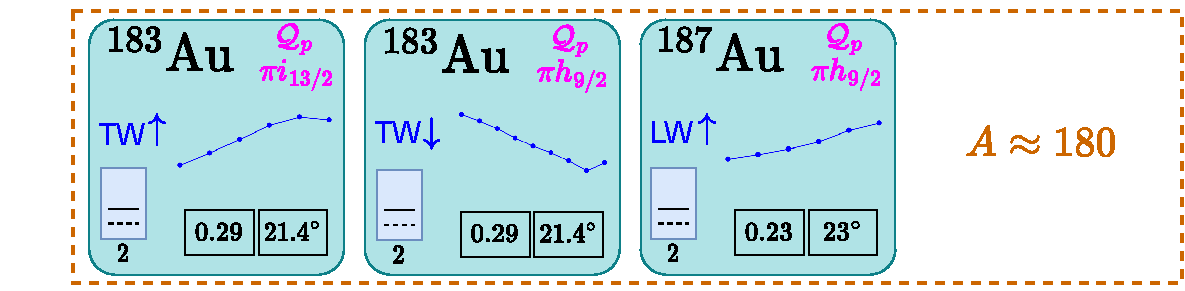
\includegraphics[width=0.99\textwidth]{figures/wobblers-chart-3.pdf}
% 	\end{figure}
% 	% \begin{figure}
% 	% 	\centering
% 	% 	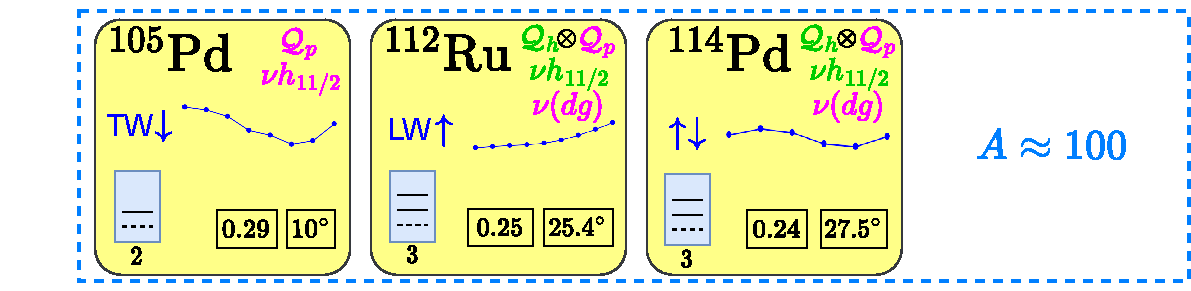
\includegraphics[width=0.99\textwidth]{figures/wobblers-chart-1.pdf}
% 	% \end{figure}
% 	\begin{beamercolorbox}[rounded=true,shadow=false, wd=\linewidth,]{block body}
% 		\centering
% 		\textcolor{black}{All diagrams and their data sources available in Chapter 3, Section 3.3.5}\\
% 		\textcolor{red}{\textbf{Presented at the Annual Meeting, FFUB, 2022.}}
% 	\end{beamercolorbox}
% \end{frame}

\subsection{Even-A case study}

\begin{frame}
	\frametitle{Wobbling Motion in $^{130}$Ba}
	\begin{columns}
		\begin{column}{0.55\textwidth}
			\faSearch\ Experimental measurements show \textbf{two} wobbling bands (\textit{Petrache et. al. 2019}).
			\begin{exampleblock}{Harmonic formalism}
				\textbf{Harmonic Approximation} (\textit{Bohr \& Mottelson, 1969}):
				\begin{align}
					E_{I,n_w}&={\color{red}A_3I(I+1)}+{\color{blue}\hbar\omega_w\left(n_w+\frac{1}{2}\right)}\nonumber,\\
					A_3&=(2\mathcal{I}_3)^{-1}\nonumber.
				\end{align}
				({\color{red}rotational term} + {\color{blue}wobbling frequency})
			\end{exampleblock}
		\end{column}
		\begin{column}{0.45\textwidth}
			\begin{figure}
				\centering
				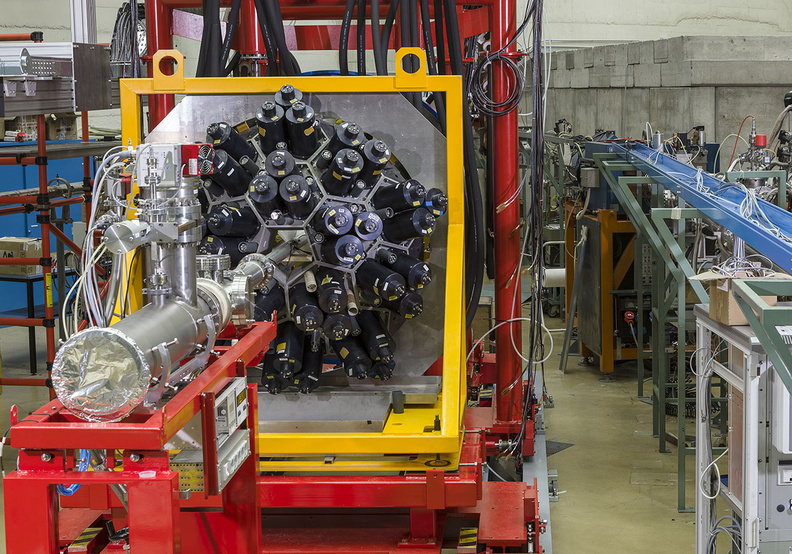
\includegraphics[width=0.99\textwidth]{figures/galileo_exp.jpg}
				{\footnotesize GALILEO, LNL, \textit{Source: lnl.infn.it}}
			\end{figure}
			{\footnotesize Fusion evaporation: $^{13}$C beam of $E=65\ \text{MeV}$ and $^{122}$Sn target.}
		\end{column}
	\end{columns}
\end{frame}

\begin{frame}
	\frametitle{Results for $^{130}$Ba}
	\begin{columns}
		\begin{column}{0.6\textwidth}
			\begin{figure}
				\centering
				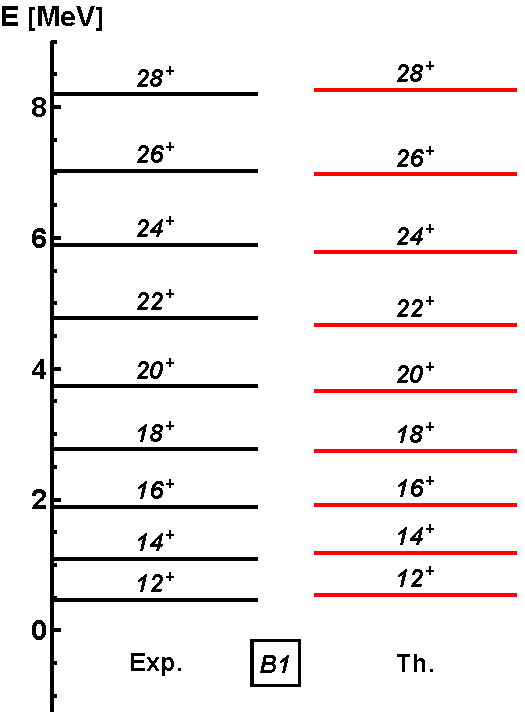
\includegraphics[width=0.49\textwidth]{figures/ba130-band1.pdf}
				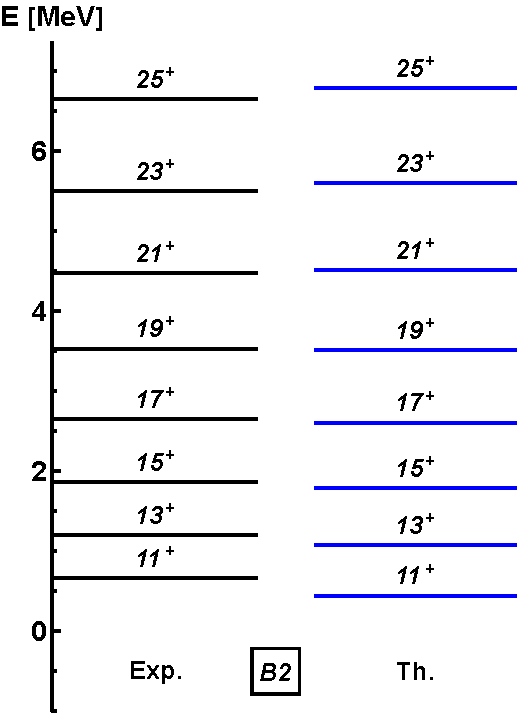
\includegraphics[width=0.49\textwidth]{figures/ba130-band2.pdf}
			\end{figure}				
		\end{column}
		\begin{column}{0.4\textwidth}
			\begin{table}
				\centering
				% \caption{The parameter set obtained from the \emph{fitting procedure}.}
				\resizebox{0.9\textwidth}{!}{%
				\begin{tabular}{cccc}
				\hline
				\multicolumn{4}{c}{$\mathcal{P}_\text{fit}$} \\ \hline \hline
				\multicolumn{1}{c}{$\mathcal{I}_1$} & \multicolumn{1}{c}{$\mathcal{I}_2$} & \multicolumn{1}{c}{$\mathcal{I}_3$} & \multicolumn{1}{c}{Unit}                     \\ \hline
				\multicolumn{1}{c}{27}              & \multicolumn{1}{c}{22}              & \multicolumn{1}{c}{\textbf{43}}              & \multicolumn{1}{c}{$\hbar^2\text{MeV}^{-1}$} \\ \hline
				\end{tabular}%
				}
				\label{table-params-ba130}
			\end{table}
			\begin{figure}
				\centering
				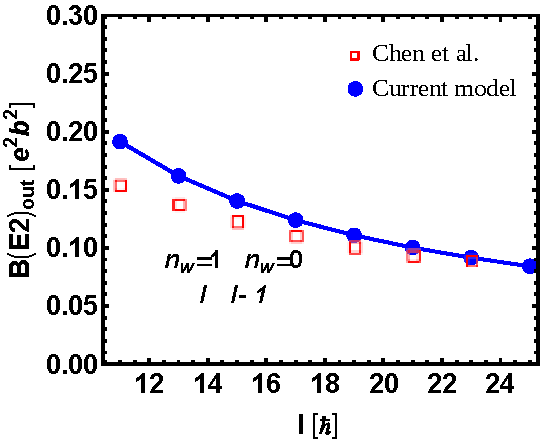
\includegraphics[width=0.99\textwidth]{figures/ba130-EM.pdf}
			\end{figure}
		\end{column}
	\end{columns}
	
	% use color box
	% \begin{tcolorbox}[colback=white, colframe=black, arc=2mm]
		% 	\centering
		% 	\begin{beamercolorbox}[rounded=true,shadow=false, wd=\linewidth,]{block body}
			% 		\centering
			% 		\textcolor{red}{\textit{Results presented at the international conference NSP, 2022, Turkey.}}
			% 	\end{beamercolorbox}
			% \end{tcolorbox}
			
	% no color box
	\begin{beamercolorbox}[rounded=true,shadow=false, wd=\linewidth,]{block body}
		\centering
		% {\footnotesize Full description: Chapter 3 (Section 3.1.2)}\\
		\textcolor{red}{\footnotesize\textbf{Results presented at the international conference NSP-2022, Turkey.}}
	\end{beamercolorbox}
\end{frame}

\begin{frame}
	\frametitle{Results for $^{130}$Ba II}
	\textbf{Excitation energies} vs. \textbf{Wobbling Energies}:
	\begin{align}
		E_\text{wob}(I_\text{even})&=E_{I,n}-E_{I,0}\ ,\nonumber \\
		E_\text{wob}(I_\text{odd})&=E_{I,n}-\frac{1}{2}\left(E_{I-1,0}+E_{I+1,0}\right) \nonumber
	\end{align}
	\vspace{-0.6cm}
	\begin{figure}
		\centering
		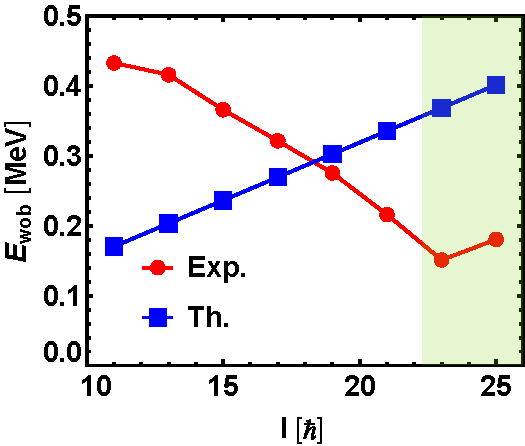
\includegraphics[scale=0.6]{figures/ba130-wobbling-energies-edited.pdf}
		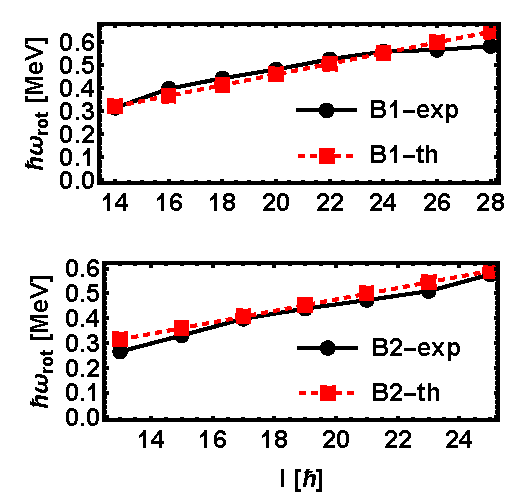
\includegraphics[scale=0.55]{figures/ba130-rotational-frequencies.pdf}
	\end{figure}
	\vspace{-0.2cm}
	\begin{beamercolorbox}[rounded=true,shadow=false, wd=\linewidth,]{block body}
		\centering
		\textcolor{red}{\small{\textbf{Results presented at the international conference NSP-2022, Turkey.}}}
	\end{beamercolorbox}
\end{frame}

\section{Wobbling Motion in Odd-A}

\begin{frame}
	\frametitle{Starting Point}
	\begin{columns}
		\begin{column}{0.6\textwidth}
			{\footnotesize \faFile\ A. A. Raduta, \textbf{R. Poenaru}, L. Gr. Ixaru, PRC, 2017} + {\footnotesize \faFile\ A. A. Raduta, \textbf{R. Poenaru}, Al. H. Raduta, JPG, 2018}$\to${\footnotesize $\mathbf{W}_0$ in the thesis.}
			\begin{exampleblock}{Framework}
				\begin{itemize}
					\item \textbf{First semi-classical description} for the $^{163}$Lu, using the \textbf{Particle-Rotor-Model} (\textit{Hamamoto, 2002}).
				\end{itemize}
			\end{exampleblock}
			\begin{alertblock}{PRM}
				\textbf{An odd-nucleon moving in a quadrupole deformed mean field generated by an even-even triaxial core.}
			\end{alertblock}
		\end{column}
		\begin{column}{0.4\textwidth}
			\begin{figure}
				\centering
				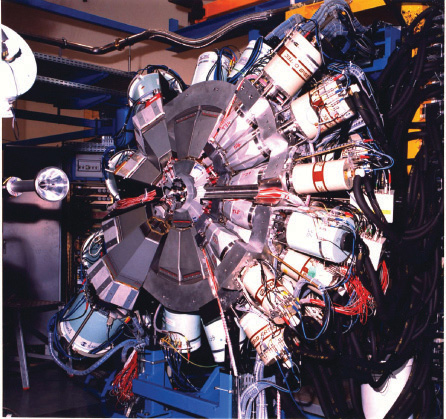
\includegraphics[width=0.99\textwidth]{figures/euroball-4.jpg}
				{\footnotesize Euroball IV, Strasbourg, \textit{Source: technologysi.stfc.ac.uk}}
			\end{figure}
			{\footnotesize Fusion evaporation: $^{29}$Si beam of $E=152\ \text{MeV}$ and $^{139}$La target.}
		\end{column}
	\end{columns}
\end{frame}

% \begin{frame}
% 	\frametitle{Overview of $\mathbf{W}_0$}
% 	\vspace{-0.3cm}
% 	\begin{columns}
% 		\begin{column}{0.6\textwidth}
% 			\begin{itemize}
% 				\item Time-Dependent Variational Principle applied on the PRM Hamiltonian
% 				\item \textbf{Phonon operators} $\rightarrow$ energies + transition probabilities
% 			\end{itemize}
% 			\vspace{-0.5cm}
% 			\begin{figure}
% 				\centering
% 				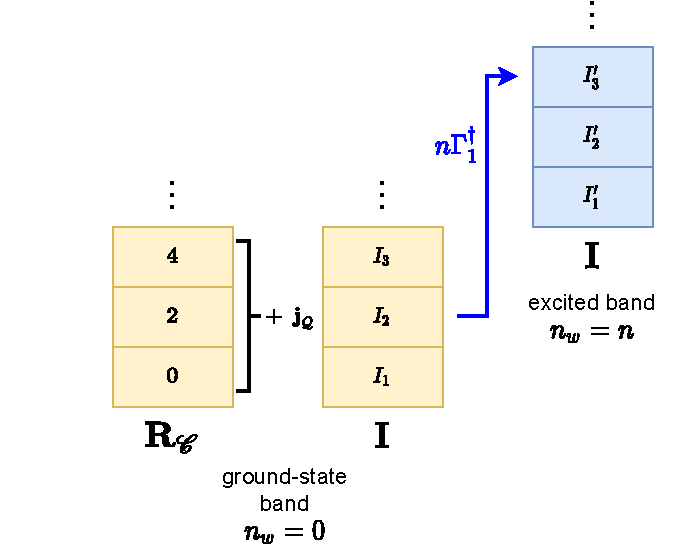
\includegraphics[width=0.9\textwidth]{figures/w0_phonon_operator.pdf}
% 			\end{figure}
% 		\end{column}
% 		\begin{column}{0.4\textwidth}
% 			\begin{figure}
% 				\centering
% 				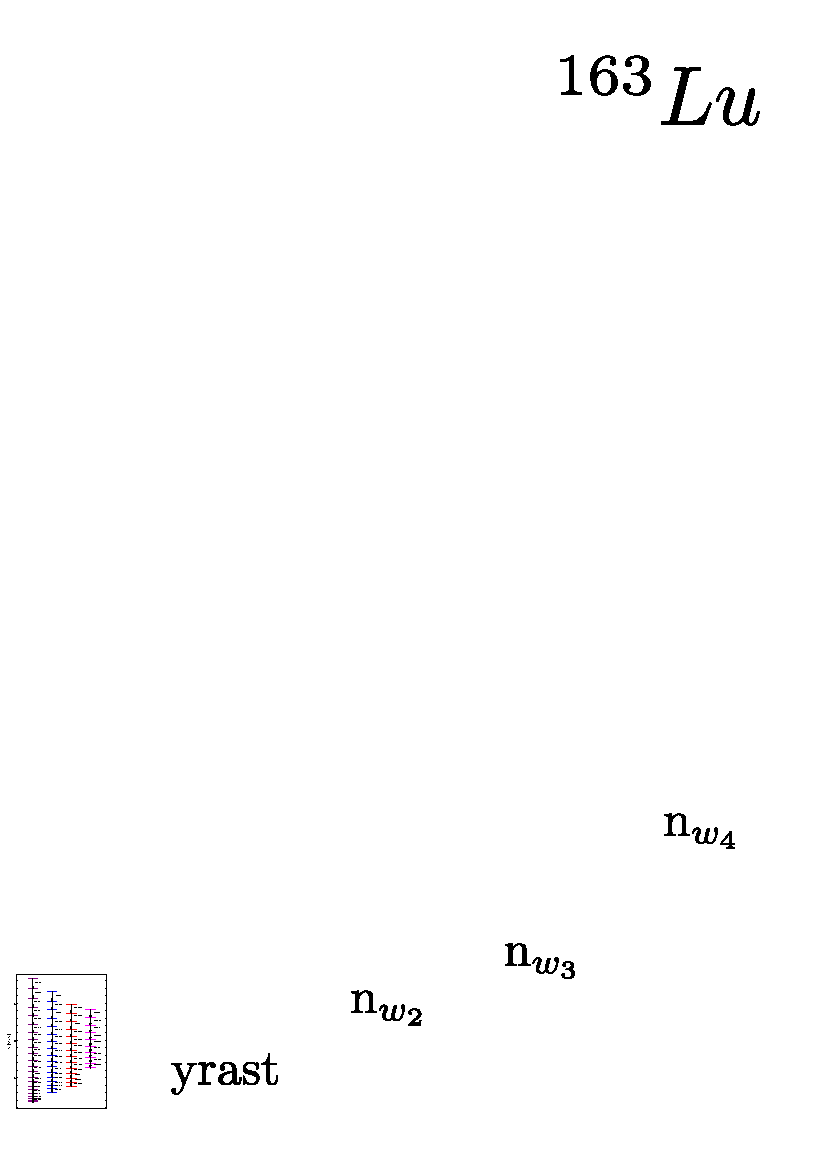
\includegraphics[width=0.99\textwidth]{figures/lu-163-exp-data.eps}
% 			\end{figure}
% 		\end{column}
% 	\end{columns}
% \end{frame}


% \begin{frame}
% 	\frametitle{Overview of $\mathbf{W}_0$ II}
% 	\begin{block}{Model characteristics}
% 		\faPlus\ Numerical data consistent with other work\\
% 		\faMinus\ TSD4: three-phonon wobbling band (disagreement with Jensen et al.)\\
% 		\faMinus\ Adopted rigid-body MOIs ("unpleasant" choice to the referees) \\
% 		\faMinus\ Deformation parameters $\beta$ and $\gamma$ taken from literature
% 	\end{block}
% 	\vspace{0.4cm}
% 	\begin{beamercolorbox}[rounded=true,shadow=false, wd=\linewidth,]{block body}
% 		\centering
% 		\textcolor{black}{\small{\textbf{Onset of a redesign $\longrightarrow$ start of a new research project}}}\\
% 		\textcolor{black}{\small{\textbf{Two new models developed presented in Chapter 4 ($\mathbf{W}_1$) and 5 ($\mathbf{W}_2$)}}}\\
% 	\end{beamercolorbox}
% \end{frame}

\subsection{Fresh-Up 1}

\begin{frame}
	\frametitle{Fresh-Up 1: $\mathbf{W}_1$}
	\vspace{-0.1cm}
	Particle-Rotor Model Hamiltonian for an odd-$A$ nucleus:	
	\vspace{-0.28cm}
	\begin{align}
		\hat{H}&={\color{red}\hat{H}_\text{rot}}+{\color{blue}\hat{H}_\text{sp}}\ ,\ {\color{red}\hat{H}_\text{rot}}={\color{red}\sum_{k=1}^3A_k(\hat{I}_k-\hat{j}_k)^2},\nonumber\\
		{\color{blue}\hat{H}_\text{sp}}&={\color{blue}\epsilon_j+\frac{V}{j(j+1)}\left[\cos\gamma\left(3\hat{j}_3^3-\mathbf{j}^2\right)-\sqrt{3}\sin\gamma\left(\hat{j}_1^2-\hat{j}_2^2\right)\right]}.\nonumber
	\end{align}
	\vspace{-0.3cm}
	$V$ - single-particle potential strength $\propto\beta_2$ (\textit{Tanabe, 2017})
	\begin{figure}
		\centering
		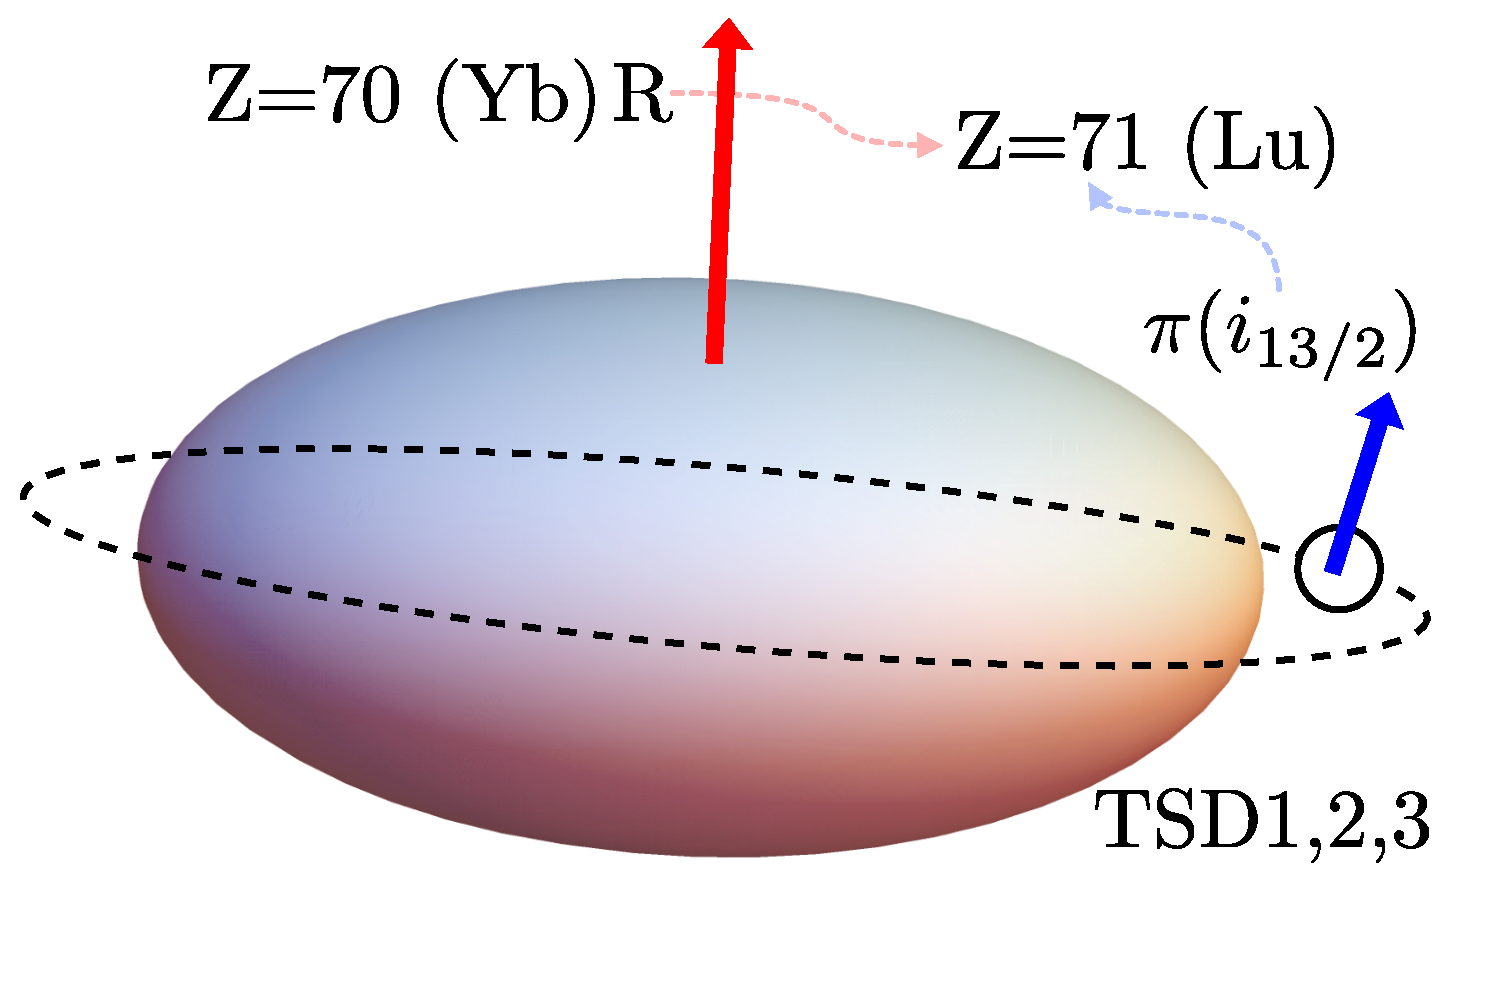
\includegraphics[scale=0.22]{figures/triaxial-shapes-oddA-1.pdf}
		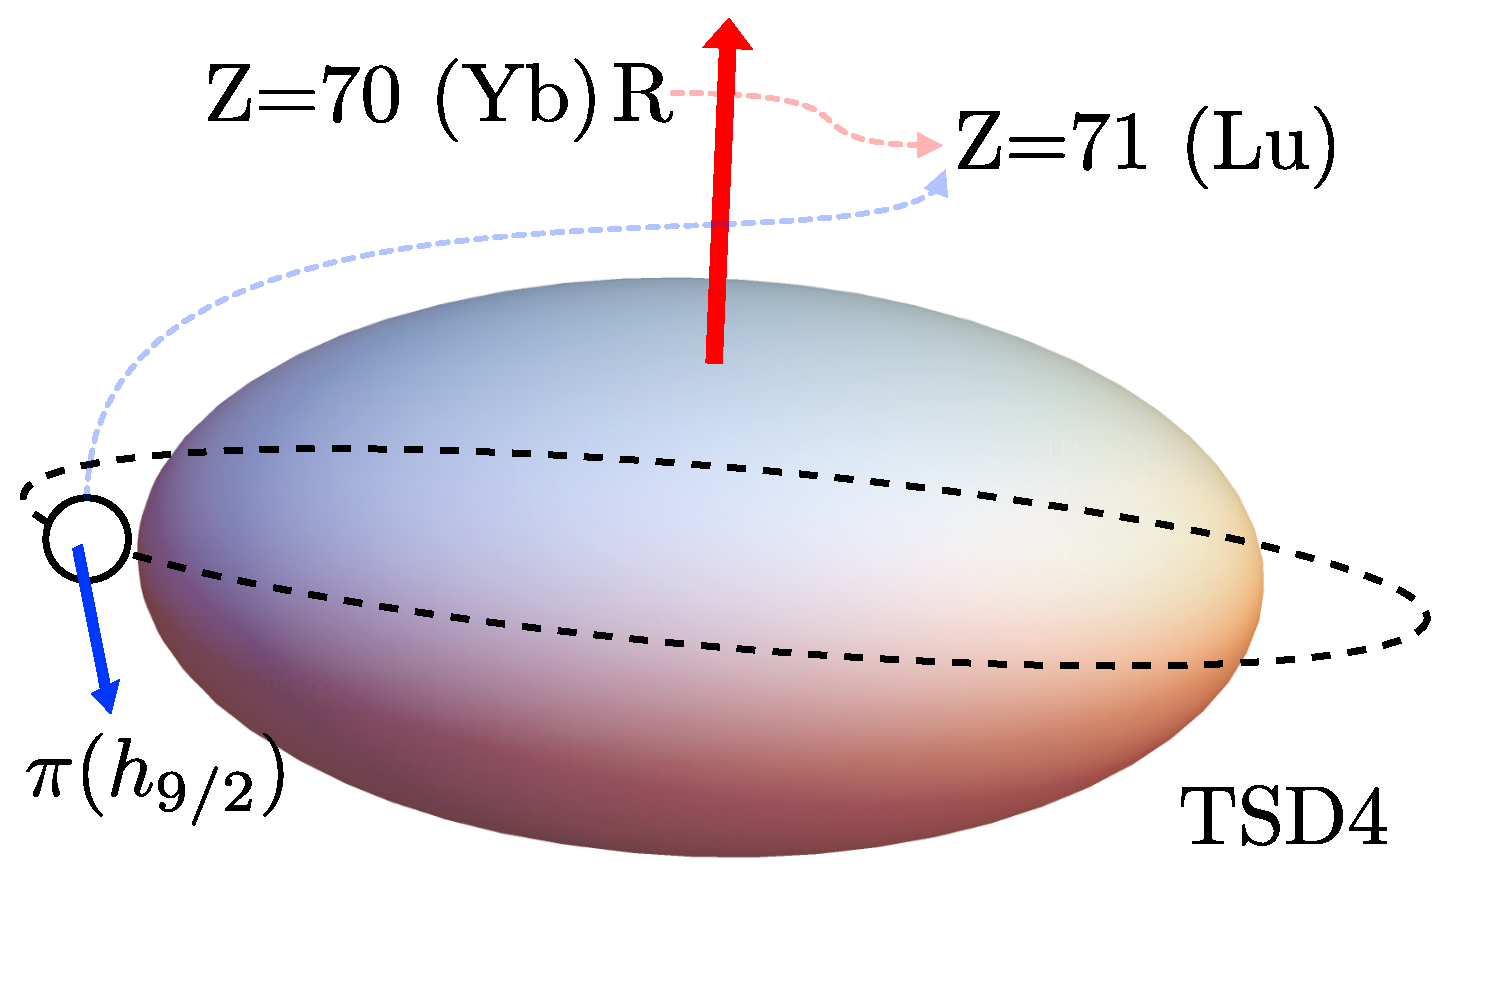
\includegraphics[scale=0.22]{figures/triaxial-shapes-oddA-2.pdf}
	\end{figure}
	\vspace{-0.5cm}
	% \begin{beamercolorbox}[rounded=true,shadow=false, wd=\linewidth,]{block body}
	% 	\centering
	% 	\textcolor{red}{\footnotesize{A. A. Raduta, \textbf{R. Poenaru}, C. M. Raduta, Phys. Rev. C 101, 2020.}}
	% \end{beamercolorbox}
	\begin{beamercolorbox}[rounded=true,shadow=false, wd=\linewidth,]{block body}
		\centering
		\textcolor{red}{\footnotesize{A.A. Raduta, \textbf{R. Poenaru}, C.M. Raduta, Journal of Physics G 47, 2020.}}
	\end{beamercolorbox}
\end{frame}

\begin{frame}
	\frametitle{Variational Principle + Eqs. of Motion}
	\begin{columns}
		\begin{column}{0.6\textwidth}
			\begin{exampleblock}{Time-Dependent Variational Equation}
				\begin{align}
					\delta&\int_0^t\bra{\Psi_{IM;j}}\hat{H}-i\frac{\partial}{\partial t'}\ket{\Psi_{IM;j}}dt'=0\nonumber\\
					\Psi_\text{trial}&\equiv\ket{\Psi_{IM;j}}=\mathcal{N}{\color{red}e^{z\hat{I}_-}}\cdot{\color{blue}e^{s\hat{j}_-}}{\color{red}\ket{IMI}}\otimes{\color{blue}\ket{jj}}\nonumber
				\end{align}
				\vspace{-0.4cm}
				\begin{itemize}
					\item {\color{red}$(z,r,\varphi,\hat{I},\ket{IMI})$} - core (rotor {\color{red}$\mathbf{R}$})
					\item {\color{blue}$(s,f,\psi,\hat{j},\ket{jj})$} - single-particle ({\color{blue}$\mathbf{j}$})
					\item $\{z,s\}\ \rightarrow$ \textbf{phase space coordinates}
				\end{itemize}
			\end{exampleblock}
		\end{column}
		\begin{column}{0.4\textwidth}
			\textbf{Constant of motion:}
			\begin{align}
				\mathcal{H}\equiv\bra{\Psi_{IM;j}}\hat{H}\ket{\Psi_{IM;j}}\nonumber
			\end{align}
			\textbf{Canonical equations of motion:}
			\begin{align}
				{\color{red}\mathcal{S}_1: \frac{\partial \mathcal{H}}{\partial r}=\dot{\varphi}\ ,\ \frac{\partial \mathcal{H}}{\partial \varphi}=-\dot{r}}\nonumber\\
				{\color{blue}\mathcal{S}_2: \frac{\partial \mathcal{H}}{\partial f}=\dot{\psi}\ ,\ \frac{\partial \mathcal{H}}{\partial \psi}=-\dot{f}}\nonumber
			\end{align}
		\end{column}
	\end{columns}
	\begin{beamercolorbox}[rounded=true,shadow=false, wd=\linewidth,]{block body}
		\centering
		\textcolor{black}{\small{The two sets of Hamilton equations are \textbf{the semi-classical description} of the initial quantal $\hat{H}$.}}
	\end{beamercolorbox}
\end{frame}


\begin{frame}
	\frametitle{Wobbling frequency}
	Solving {\color{red}$\mathcal{S}_1$} and {\color{blue}$\mathcal{S}_2$} leads to the algebraic equation:
	\begin{align}
		\Omega^4+B\Omega^2+C=0\nonumber
	\end{align}
	four solutions $\longrightarrow$ \textbf{only two are real}:
	\begin{align}
		\Omega_{1,2}=\left[\frac{1}{2}\left(-B\mp\sqrt{B^2-4C}\right)\right]^{1/2}\nonumber
	\end{align}
	\begin{itemize}
		\item {\color{red}$\Omega_1$}: wobbling frequency of the {\color{red}even-$A$ core $\mathbf{R}$}
		\item {\color{blue}$\Omega_2$}: wobbling frequency of the {\color{blue}odd-nucleon $\mathbf{j}$}
		\item \textbf{Two wobbling phonon numbers: {\color{red}$n_{w_1}$} and {\color{blue}$n_{w_2}$}}
	\end{itemize}
	\begin{beamercolorbox}[rounded=true,shadow=false, wd=\linewidth,]{block body}
		\centering
		\textcolor{red}{\footnotesize{A.A. Raduta, \textbf{R. Poenaru}, C.M. Raduta, Journal of Physics G 47, 2020.}}
	\end{beamercolorbox}
	% \begin{beamercolorbox}[rounded=true,shadow=false, wd=\linewidth,]{block body}
	% 	\centering
	% 	\textcolor{red}{\footnotesize{A. A. Raduta, \textbf{R. Poenaru}, C. M. Raduta, Phys. Rev. C 101, 2020.}}
	% \end{beamercolorbox}
\end{frame}

\begin{frame}
	\frametitle{Energy spectrum}
	\begin{exampleblock}{Spectra of odd-A nuclei within $\mathbf{W}_1$}
		\begin{align}
			E_{I,n_1,n_2}=\epsilon_j+\mathcal{H}_\text{min}^I+\mathcal{F}_{n_{w_1}n_{w_2}}^I\nonumber
			\label{tsd-bands-general-spectrum}
		\end{align}
	\end{exampleblock}
	\begin{itemize}
		\item Phonon factor:
		\begin{align}
			\mathcal{F}_{n_{w_1}n_{w_2}}^I&={\color{red}\hbar\Omega_1^I\left(n_{w_1}+\frac{1}{2}\right)}+{\color{blue}\hbar\Omega_2^I\left(n_{w_2}+\frac{1}{2}\right)}\nonumber
		\end{align}
		\item $\mathcal{H}_\text{min}^I$ - Classical Energy Function taken in its minimum point: $p_0=(0,I;0,j)$.
		\item $\epsilon_j$ - single-particle energy
	\end{itemize}
\end{frame}

\begin{frame}
	\frametitle{A new interpretation for TSD1 and TSD2}
	\begin{exampleblock}{Previous models}
		$TSD1=$ zero-phonon wobbling band\\
		$TSD2=$ one-phonon wobbling band...
	\end{exampleblock}
	\begin{alertblock}{Redefinition}
		$TSD1$ and $TSD2$ are \textbf{Signature Partner Bands} (in favor of Ultimate Cranker calculations, \textit{Jensen, 2004}).
		\begin{align}
			\left(\alpha_{fav}=+\frac{1}{2}\right): \{TSD1\}&\equiv\left\{\left[0^+,2^+,4^+,\dots\right] \otimes [j^\pi=13/2^+]\right\}\nonumber\\
			\left(\alpha_{unfav}=-\frac{1}{2}\right): \{TSD2\}&\equiv\left\{\left[1^+,3^+,5^+,\dots\right] \otimes [j^\pi=13/2^+]\right\}\nonumber
		\end{align}
		$TSD4$ is a \textbf{ground-state wobbling band}, $\pi(h_{9/2})$ configuration.
	\end{alertblock}
	% \begin{beamercolorbox}[rounded=true,shadow=false, wd=\linewidth,]{block body}
	% 	\centering
	% 	\textcolor{red}{\footnotesize{A. A. Raduta, \textbf{R. Poenaru}, C. M. Raduta, Phys. Rev. C 101, 2020.}}
	% \end{beamercolorbox}
	\begin{beamercolorbox}[rounded=true,shadow=false, wd=\linewidth,]{block body}
		\centering
		\textcolor{red}{\footnotesize{A.A. Raduta, \textbf{R. Poenaru}, C.M. Raduta, Journal of Physics G 47, 2020.}}
	\end{beamercolorbox}
\end{frame}

\begin{frame}
	\frametitle{A new band structure for $^{163}$Lu}
	\begin{table}
		\centering
		\resizebox{\textwidth}{!}{%
		\begin{tabular}{ccccccc}
		\hline
		Band & Spins & $\pi$ & $\alpha$ & $\pi(l_j)$ & $\mathbf{W_0}$: $\mathscr{C}+\mathcal{Q}_p$ & $\mathbf{W_1}$: $\mathscr{C}+\mathcal{Q}_p$ \\ \hline \hline
		TSD1 & $13/2,17/2 \dots 97/2$ & $+$ & $+1/2$ & $\pi(i_{13/2})$ & $0^+,2^+,4^+,\dots$ & $0^+,2^+,4^+,\dots$ \\ \hline
		TSD2 & $27/2,31/2 \dots 91/2$ & $+$ & $-1/2$ & $\pi(i_{13/2})$ & $\text{TSD1}+1\Gamma^\dagger$ & $1^+,3^+,5^+,\dots$ \\ \hline
		TSD3 & $33/2,37/2 \dots 85/2$ & $+$ & $+1/2$ & $\pi(i_{13/2})$ & $\text{TSD1}+2\Gamma^\dagger$ & $\text{TSD2}+\Gamma^\dagger$ \\ \hline
		TSD4 & $47/2,51/2 \dots 83/2$ & $-$ & $-1/2$ & $\pi(h_{9/2})$  & $\text{TSD1}+3\Gamma^\dagger$ & $1^+,3^+,5^+,\dots$ \\ \hline
		\end{tabular}%
		}
	\end{table}
	\begin{table}
		\centering
		\resizebox{\textwidth}{!}{%
		\begin{tabular}{ccccccc}
		\hline
		Bands & $n_{w_1}$ & $n_{w_2}$ & $\mathcal{F}_{n_{w_1}n_{w_2}}^I$ & $I_0$    & $I_t$    & $\mathcal{Q}$    \\ \hline \hline 
		TSD1  & $0$       & $0$       & $\mathcal{F}_{00}^I=\frac{1}{2}\left(\Omega_1^I+\Omega_2^I\right)$ & $13/2^+$ & $97/2^+$ & $j^\pi=13/2^+\stackrel{not}{\equiv}\mathcal{Q}_1$ \\ \hline
		TSD2  & $\mathbf{0}$       & $\mathbf{0}$       & $\mathcal{F}_{00}^I=\frac{1}{2}\left(\Omega_1^I+\Omega_2^I\right)$ & $27/2^+$ & $91/2^+$ & $j^\pi=13/2^+\stackrel{not}{\equiv}\mathcal{Q}_1$ \\ \hline
		TSD3  & $1$       & $0$       & $\mathcal{F}_{10}^{I-1}=\frac{3}{2}\Omega_1^{I-1}+\frac{1}{2}\Omega_2^{I-1}$ & $33/2^+$ & $85/2^+$ & $j^\pi=13/2^+\stackrel{not}{\equiv}\mathcal{Q}_1$ \\ \hline
		\textbf{TSD4}  & $\mathbf{0}$       & $\mathbf{0}$       & $\mathcal{F}_{00}^I=\frac{1}{2}\left(\Omega_1^I+\Omega_2^I\right)$ & $47/2^-$ & $83/2^-$ & $j^\pi=9/2^-\stackrel{not}{\equiv}\mathcal{Q}_2$  \\ \hline
		\end{tabular}%
		}
	\end{table}
	\vspace{-0.3cm}
	\begin{beamercolorbox}[rounded=true,shadow=false, wd=\linewidth,]{block body}
		\centering
		\textcolor{red}{\footnotesize{A.A. Raduta, \textbf{R. Poenaru}, C.M. Raduta, Journal of Physics G 47, 2020.}}
	\end{beamercolorbox}
\end{frame}

\begin{frame}
	\frametitle{Extension to $A\approx160$ mass region}
	\vspace{-0.4cm}
	The model was further applied to the other Lu isotopes.
	\vspace{-0.5cm}
	\begin{table}
		\centering
		\resizebox{\textwidth}{!}{%
		\begin{tabular}{cccccc}
			\hline
			$^{161}$Lu Bands & Spins                        & $\mathcal{Q}$ & $\mathscr{C}$  & $(n_{w_1},n_{w_2})$ & $I_b$                   \\ \hline \hline
			TSD1 & $21/2^+,25/2^+,\dots,89/2^+$ & $j^\pi=13/2^+$  & $4^+,6^+,8^+\dots$   & $(0,0)$             & \multirow{2}{*}{$21/2$} \\ \cline{1-5}
			TSD2 & $31/2^+,35/2^+,\dots,79/2^+$ & $j^\pi=13/2^+$  & $9^+,11^+,13^+\dots$ & $(0,0)$             &                         \\ \hline
		\end{tabular}%
		}
		\label{lu-161-experimental-data-table}
	\end{table}
	\vspace{-0.5cm}
	\begin{table}
		\centering
		\resizebox{\textwidth}{!}{%
		\begin{tabular}{cccccc}
			\hline
			$^{165}$Lu Bands & Spins                        & $\mathcal{Q}$ & $\mathscr{C}$         & $(n_{w_1},n_{w_2})$ & $I_b$                   \\ \hline \hline
			TSD1 & $25/2^+,29/2^+,\dots,89/2^+$ & $j^\pi=13/2^+$  & $6^+,8^+,10^+\dots$   & $(0,0)$             & \multirow{3}{*}{$25/2$} \\ \cline{1-5}
			TSD2 & $35/2^+,39/2^+,\dots,91/2^+$ & $j^\pi=13/2^+$  & $11^+,13^+,15^+\dots$ & $(0,0)$             &                         \\ \cline{1-5}
			TSD3 & $41/2^+,45/2^+,\dots,81/2^+$ & $j^\pi=13/2^+$  & $\text{TSD2}+\Gamma^\dagger$ & $(1,0)$             &                         \\ \hline
		\end{tabular}%
		}
		\label{lu-165-experimental-data-table}
	\end{table}
	\vspace{-0.5cm}
	\begin{table}
		\centering
		\resizebox{\textwidth}{!}{%
		\begin{tabular}{cccccc}
			\hline
			$^{167}$Lu Bands & Spins                        & $\mathcal{Q}$ & $\mathscr{C}$         & $(n_{w_1},n_{w_2})$ & $I_b$                   \\ \hline \hline
			TSD1 & $25/2^+,29/2^+,\dots,89/2^+$ & $j^\pi=13/2^+$  & $6^+,8^+,10^+\dots$   & $(0,0)$             & \multirow{2}{*}{$25/2$} \\ \cline{1-5}
			TSD2 & $35/2^+,39/2^+,\dots,91/2^+$ & $j^\pi=13/2^+$  & $11^+,13^+,15^+\dots$ & $(0,0)$             &                         \\ \hline
		\end{tabular}%
		}
		\label{lu-167-experimental-data-table}
	\end{table}
	\begin{beamercolorbox}[rounded=true,shadow=false, wd=\linewidth,]{block body}
		\centering
		\textcolor{red}{\footnotesize{A. A. Raduta, \textbf{R. Poenaru}, C. M. Raduta, Phys. Rev. C 101, 2020.}}
	\end{beamercolorbox}
\end{frame}

\begin{frame}
	\frametitle{$\mathbf{W}_1$ | Numerical Results}
	Free parameters in the model $\rightarrow\mathcal{P}_\text{fit}=\left[\mathcal{I}_1,\mathcal{I}_2,\mathcal{I}_3,V,\gamma\right]$.
	\begin{block}{Fitting procedure}
		\vspace{-0.4cm}
		\begin{align}
			\chi^2=\frac{1}{N_T}\sum_i\frac{\left(E_\text{exp}^{(i)}-E_\text{th}^{(i)}\right)^2}{E_\text{exp}^{(i)}}\nonumber
		\end{align}
		$^{163}$Lu-TSD4: separate fitting procedure (different nucleon configuration)
	\end{block}
	\begin{table}
		\centering
		\resizebox{\textwidth}{!}{%
		\begin{tabular}{ccccccccc}
		\hline
		Isotope &  Bands & $\mathcal{I}_1$ $\left[\hbar^2/\text{MeV}\right]$ & $\mathcal{I}_2$ $\left[\hbar^2/\text{MeV}\right]$ & $\mathcal{I}_3$ $\left[\hbar^2/\text{MeV}\right]$ & $V$ [MeV] & $\gamma$ [$^\circ$] & n.o.s & $E_\text{rms}$ [MeV] \\ \hline \hline
		$^{161}$Lu & TSD1-2 & 87.555 & 2.773  & 22.744 & 2.933 & 20    & 29 & 0.168 \\
		$^{163}$Lu & TSD1-3 & 63.2   & 20     & 10     & 3.1   & 17    & 52 & 0.264 \\
					& TSD4   & 67     & 34.5   & 50     & 0.7   & 17    & 10 & 0.057 \\
		$^{165}$Lu & TSD1-3 & 77.295 & 16.184 & 4.399  & 1.673 & 20    & 42 & 0.125 \\
		$^{167}$Lu & TSD1-2 & 87.032 & 10.895 & 3.758  & 8.167 & 19.48 & 30 & 0.165 \\
		\hline
		\end{tabular}%
		}
	\end{table}
	\begin{beamercolorbox}[rounded=true,shadow=false, wd=\linewidth,]{block body}
		\centering
		\textcolor{red}{\footnotesize{A. A. Raduta, \textbf{R. Poenaru}, C. M. Raduta, Phys. Rev. C 101, 2020.}}
	\end{beamercolorbox}
\end{frame}

\begin{frame}
	\frametitle{Graphical representation for MOIs and V}
	\vspace{-0.5cm}
	\begin{figure}
		\centering
		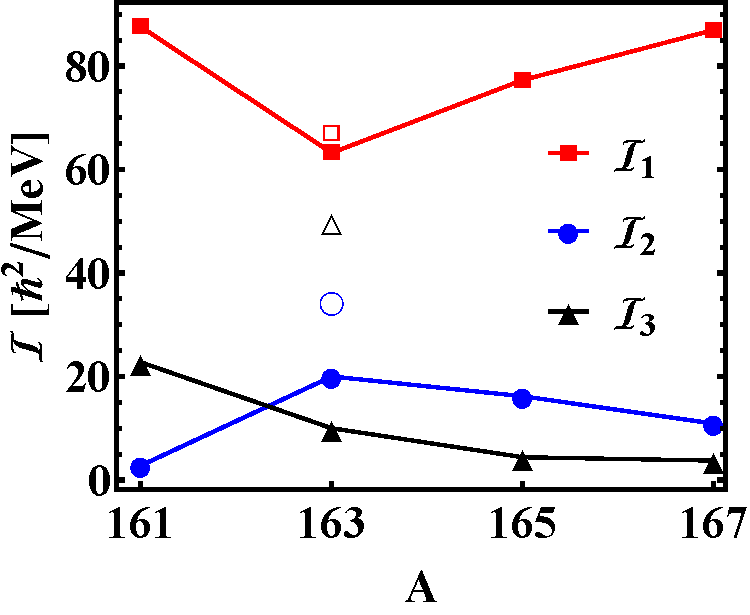
\includegraphics[scale=0.46]{figures/fig1_moivalues.pdf}
		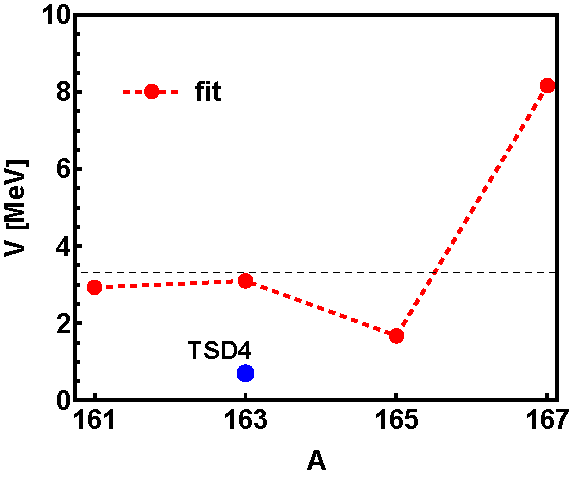
\includegraphics[scale=0.61]{figures/V-param-fitting.pdf}
		\vspace{-0.2cm}
		% \caption{Fitted values for the MOIs and the single-particle potential strength.}
	\end{figure}
	% \vspace{-0.5cm}
	$V\approx 3$ MeV $\rightarrow$ agreement with other calculations (\textit{Tanabe, 2017})
	\begin{beamercolorbox}[rounded=true,shadow=false, wd=\linewidth,]{block body}
		\centering
		\textcolor{red}{\footnotesize{A. A. Raduta, \textbf{R. Poenaru}, C. M. Raduta, Phys. Rev. C 101, 2020.}}
	\end{beamercolorbox}
\end{frame}

\begin{frame}
	\frametitle{Excitation Energies | $^{161,167}$Lu}
	\begin{figure}
		\centering
		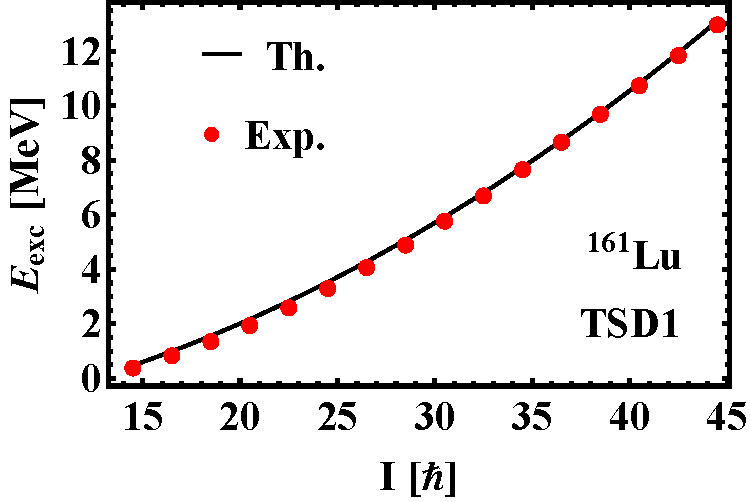
\includegraphics[width=0.41\textwidth]{figures/Lu-exp-energies/fig2a_lu161.pdf}
		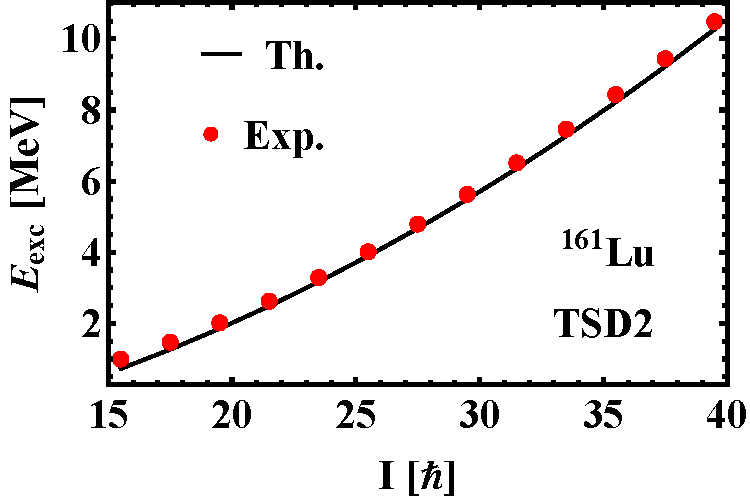
\includegraphics[width=0.41\textwidth]{figures/Lu-exp-energies/fig2b_lu161.pdf}
	\end{figure}
	\vspace{-0.5cm}
	\begin{figure}
		\centering
		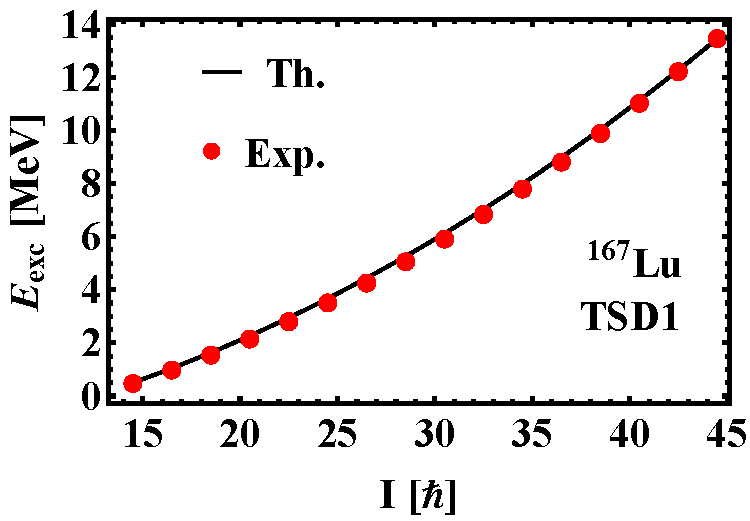
\includegraphics[width=0.41\textwidth]{figures/Lu-exp-energies/fig5a_lu167.pdf}
		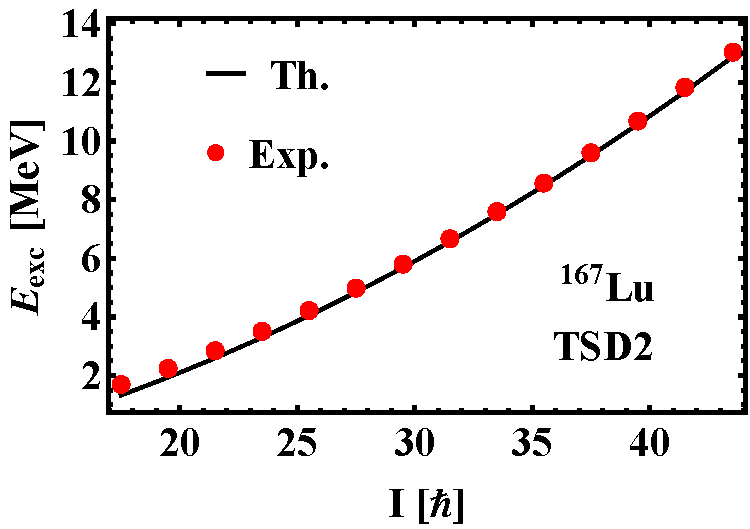
\includegraphics[width=0.41\textwidth]{figures/Lu-exp-energies/fig5b_lu167.pdf}
	\end{figure}
	\vspace{-0.2cm}
	\begin{beamercolorbox}[rounded=true,shadow=false, wd=\linewidth,]{block body}
		\centering
		\textcolor{red}{\footnotesize{A. A. Raduta, \textbf{R. Poenaru}, C. M. Raduta, Phys. Rev. C 101, 2020.}}
	\end{beamercolorbox}
\end{frame}

\begin{frame}
	\frametitle{Excitation Energies | $^{163}$Lu}
	\begin{figure}
		\centering
		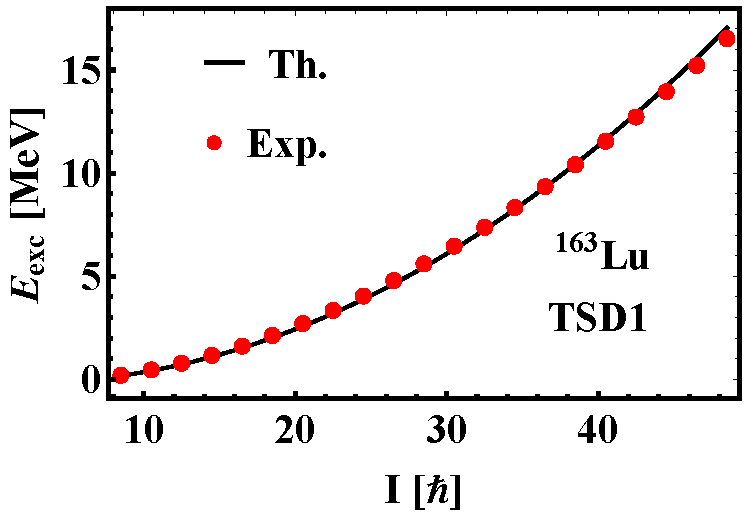
\includegraphics[width=0.41\textwidth]{figures/Lu-exp-energies/fig3a_lu163.pdf}
		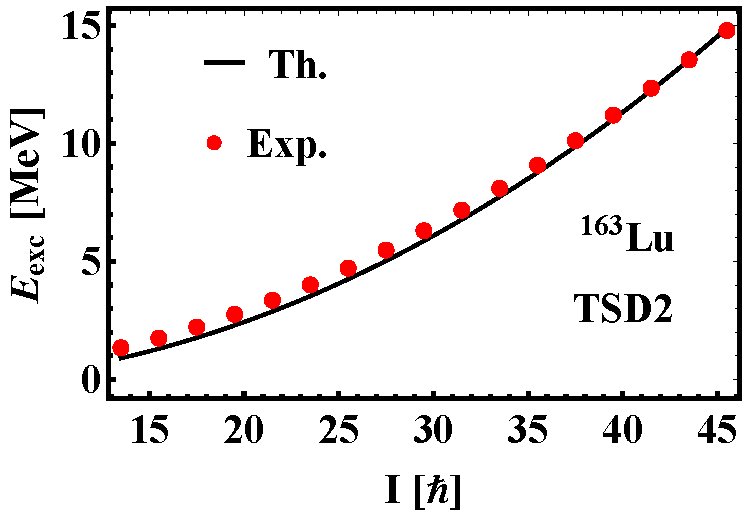
\includegraphics[width=0.41\textwidth]{figures/Lu-exp-energies/fig3b_lu163.pdf}
	\end{figure}
	\vspace{-0.4cm}
	\begin{figure}
		\centering
		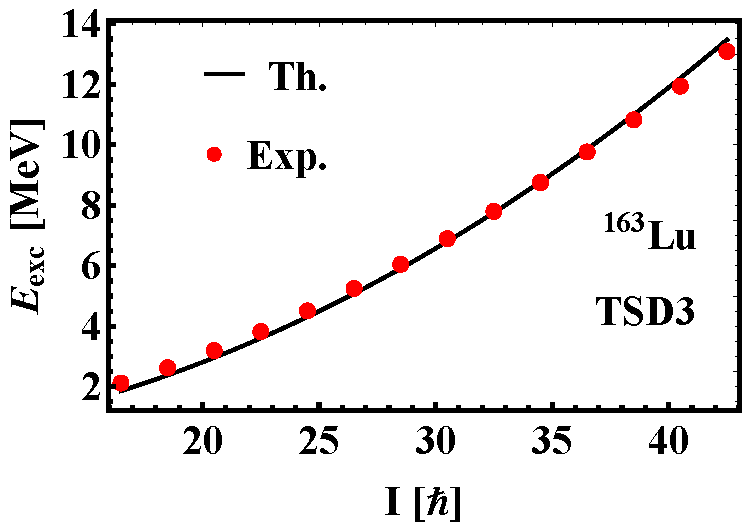
\includegraphics[width=0.41\textwidth]{figures/Lu-exp-energies/fig3c_lu163.pdf}
		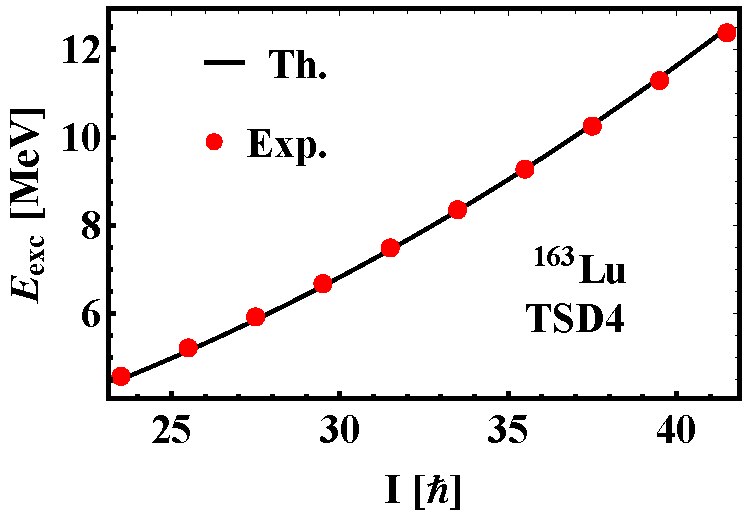
\includegraphics[width=0.41\textwidth]{figures/Lu-exp-energies/fig3d_lu163.pdf}
	\end{figure}
	\vspace{-0.2cm}
	\begin{beamercolorbox}[rounded=true,shadow=false, wd=\linewidth,]{block body}
		\centering
		\textcolor{red}{\footnotesize{A. A. Raduta, \textbf{R. Poenaru}, C. M. Raduta, Phys. Rev. C 101, 2020.}}
	\end{beamercolorbox}
\end{frame}

\begin{frame}
	\frametitle{Excitation Energies | $^{165}$Lu}
	\vspace{-0.2cm}
	\begin{figure}
		\centering
		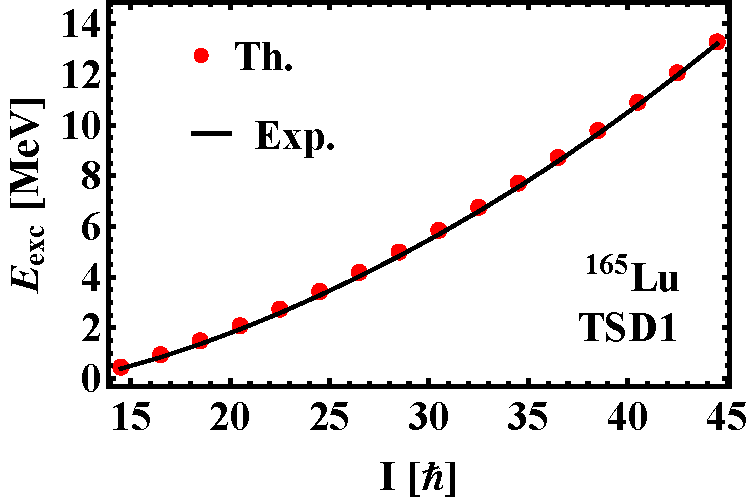
\includegraphics[width=0.41\textwidth]{figures/Lu-exp-energies/fig4a_lu165.pdf}
		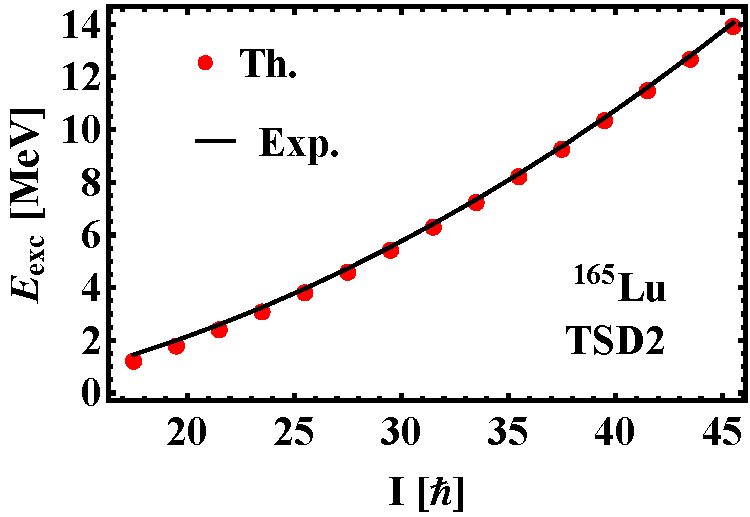
\includegraphics[width=0.41\textwidth]{figures/Lu-exp-energies/fig4b_lu165.pdf}
		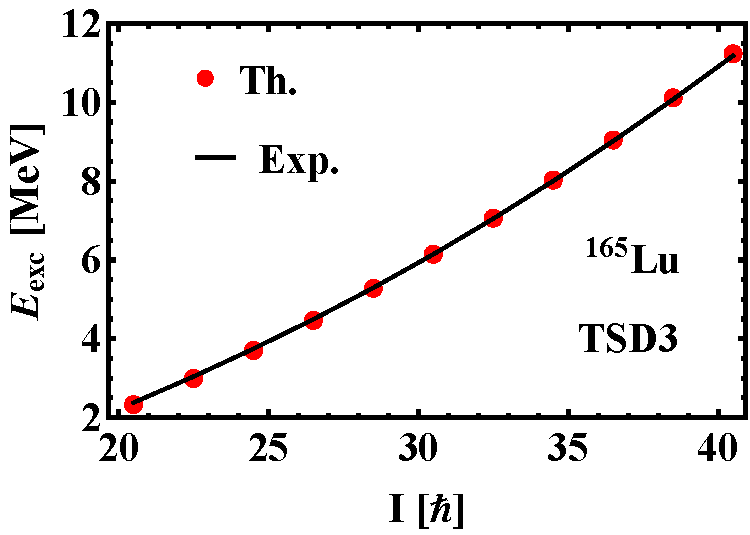
\includegraphics[width=0.41\textwidth]{figures/Lu-exp-energies/fig4c_lu165.pdf}
	\end{figure}
	\vspace{-0.2cm}
	\begin{beamercolorbox}[rounded=true,shadow=false, wd=\linewidth,]{block body}
		\centering
		\textcolor{red}{\footnotesize{A. A. Raduta, \textbf{R. Poenaru}, C. M. Raduta, Phys. Rev. C 101, 2020.}}
	\end{beamercolorbox}
\end{frame}

\begin{frame}
	\frametitle{Alignment | $^{161,167}$Lu}
	\vspace{-0.5cm}
	\begin{align}
		i_x=&I-I_\text{ref}\ ,\nonumber\\
		I_\text{ref}=&\mathcal{I}_0\omega+\mathcal{I}_1\omega^3\ .\nonumber
	\end{align}
	\vspace{-0.5cm}
	\begin{figure}
		\centering
		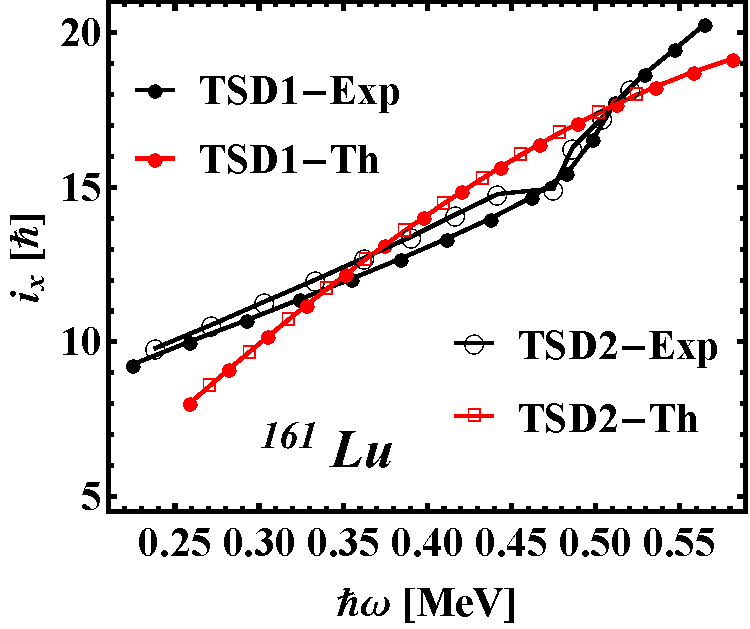
\includegraphics[width=0.45\textwidth]{figures/Lu-exp-energies/fig7.pdf}
		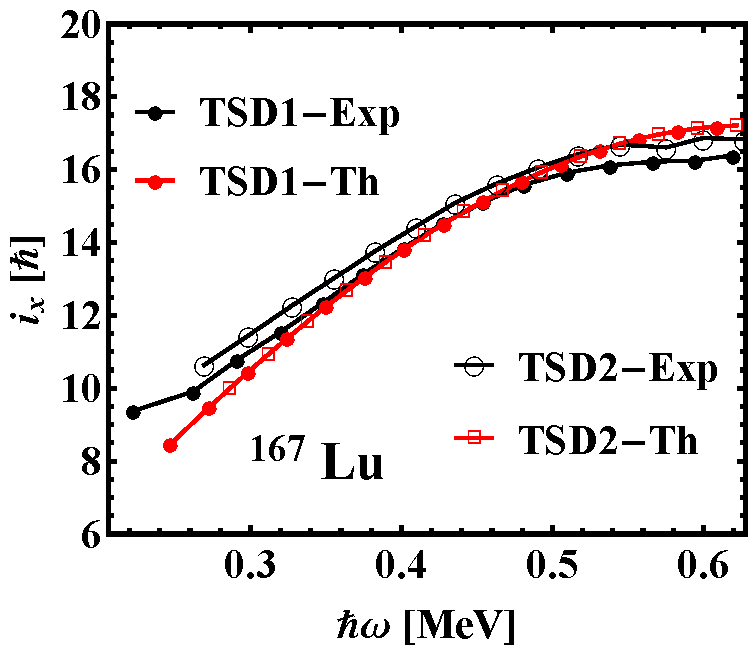
\includegraphics[width=0.45\textwidth]{figures/Lu-exp-energies/fig10.pdf}
	\end{figure}
	\begin{beamercolorbox}[rounded=true,shadow=false, wd=\linewidth,]{block body}
		\centering
		\textcolor{red}{\footnotesize{A. A. Raduta, \textbf{R. Poenaru}, C. M. Raduta, Phys. Rev. C 101, 2020.}}
	\end{beamercolorbox}
\end{frame}

\begin{frame}
	\frametitle{Alignment | $^{163}$Lu}
	\begin{figure}
		\centering
		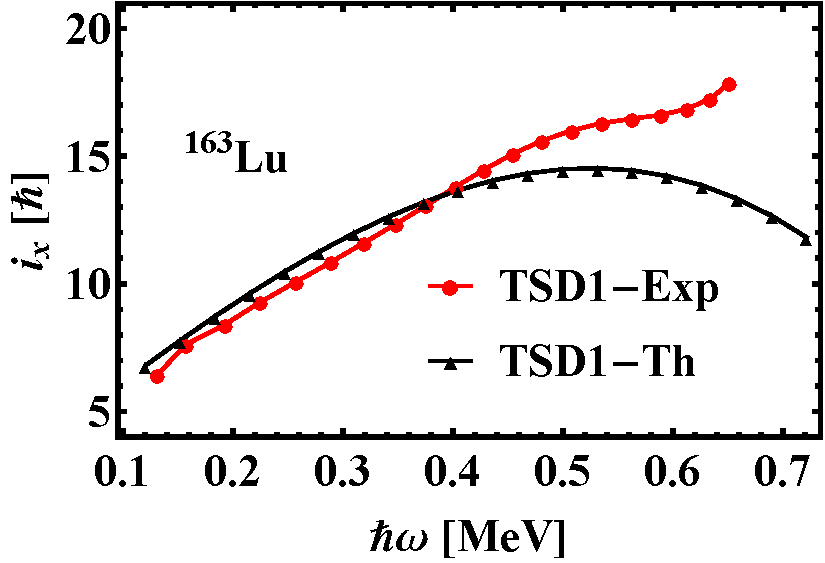
\includegraphics[width=0.4\textwidth]{figures/Lu-exp-energies/fig8a_lu163.pdf}
		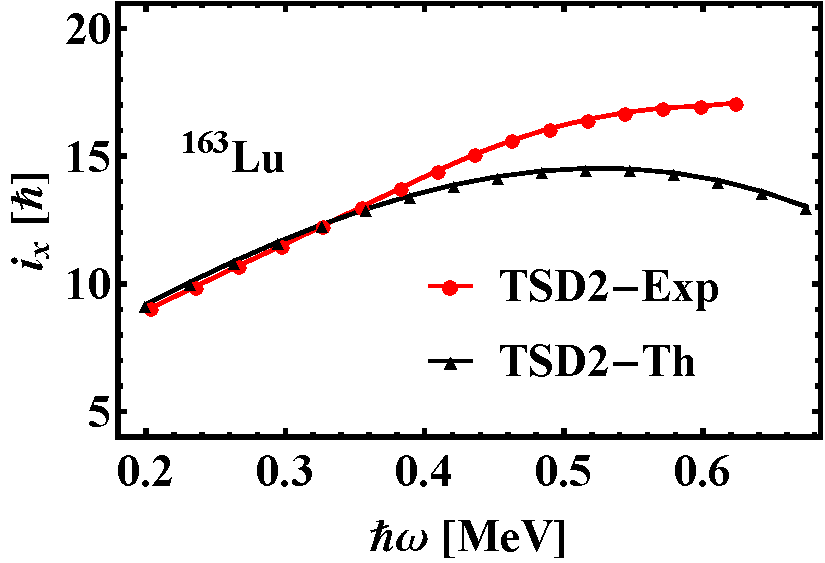
\includegraphics[width=0.4\textwidth]{figures/Lu-exp-energies/fig8b_lu163.pdf}
		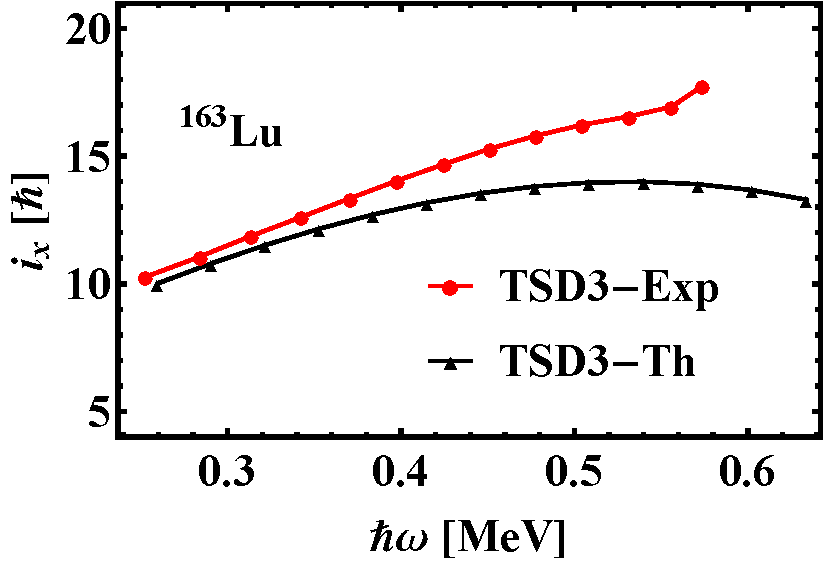
\includegraphics[width=0.4\textwidth]{figures/Lu-exp-energies/fig8c_lu163.pdf}
		\includegraphics[width=0.4\textwidth]{figures/Lu-exp-energies/fig8d_lu163.pdf}
	\end{figure}
	\begin{beamercolorbox}[rounded=true,shadow=false, wd=\linewidth,]{block body}
		\centering
		\textcolor{red}{\footnotesize{A. A. Raduta, \textbf{R. Poenaru}, C. M. Raduta, Phys. Rev. C 101, 2020.}}
	\end{beamercolorbox}
\end{frame}

\begin{frame}
	\frametitle{Alignment | $^{165}$Lu}
	\begin{figure}
		\centering
		\includegraphics[width=0.49\textwidth]{figures/Lu-exp-energies/fig9a_lu165.pdf}
		\includegraphics[width=0.49\textwidth]{figures/Lu-exp-energies/fig9b_lu165.pdf}
	\end{figure}
	\begin{beamercolorbox}[rounded=true,shadow=false, wd=\linewidth,]{block body}
		\centering
		\textcolor{red}{\footnotesize{A. A. Raduta, \textbf{R. Poenaru}, C. M. Raduta, Phys. Rev. C 101, 2020.}}
	\end{beamercolorbox}
\end{frame}

\begin{frame}
	\frametitle{Dynamic Moment of Inertia | $^{161,167}$Lu}
	\vspace{-0.5cm}
	\begin{align}
		\mathcal{I}^{(2)}(I)=\hbar\frac{\text{d}I_x}{\text{d}\omega}=\hbar^2\left(\frac{\text{d}^2E}{\text{d}I_x^2}\right)^{-1}\nonumber
	\end{align}
	\vspace{-0.5cm}
	\begin{figure}
		\centering
		\includegraphics[width=0.49\textwidth]{figures/Lu-exp-energies/fig15_lu161.pdf}
		\includegraphics[width=0.49\textwidth]{figures/Lu-exp-energies/fig18_lu167.pdf}
	\end{figure}
	\begin{beamercolorbox}[rounded=true,shadow=false, wd=\linewidth,]{block body}
		\centering
		\textcolor{red}{\footnotesize{A. A. Raduta, \textbf{R. Poenaru}, C. M. Raduta, Phys. Rev. C 101, 2020.}}
	\end{beamercolorbox}
\end{frame}

\begin{frame}
	\frametitle{Dynamic Moment of Inertia | $^{163}$Lu}
	\begin{figure}
		\centering
		\includegraphics[width=0.49\textwidth]{figures/Lu-exp-energies/fig16a_lu163.pdf}
		\includegraphics[width=0.49\textwidth]{figures/Lu-exp-energies/fig16b_lu163.pdf}
	\end{figure}
	\begin{beamercolorbox}[rounded=true,shadow=false, wd=\linewidth,]{block body}
		\centering
		\textcolor{red}{\footnotesize{A. A. Raduta, \textbf{R. Poenaru}, C. M. Raduta, Phys. Rev. C 101, 2020.}}
	\end{beamercolorbox}
\end{frame}

\begin{frame}
	\frametitle{Dynamic Moment of Inertia | $^{165}$Lu}
	\begin{figure}
		\centering
		\includegraphics[width=0.49\textwidth]{figures/Lu-exp-energies/fig17a_lu165.pdf}
		\includegraphics[width=0.49\textwidth]{figures/Lu-exp-energies/fig17b_lu165.pdf}
	\end{figure}
	\begin{beamercolorbox}[rounded=true,shadow=false, wd=\linewidth,]{block body}
		\centering
		\textcolor{red}{\footnotesize{A. A. Raduta, \textbf{R. Poenaru}, C. M. Raduta, Phys. Rev. C 101, 2020.}}
	\end{beamercolorbox}
\end{frame}

\begin{frame}
	\frametitle{Electromagnetic Calculations}
	\begin{figure}
		\centering
		\includegraphics[width=0.475\textwidth]{figures/BE2inout-1.pdf}
		\includegraphics[width=0.49\textwidth]{figures/BE2inout-2.pdf}
		\caption{E2 Branching ratio. \textbf{Left}: $^{163}$Lu (TSD2) \textbf{Right}: $^{165}$Lu (TSD2).}
	\end{figure}
	\begin{beamercolorbox}[rounded=true,shadow=false, wd=\linewidth,]{block body}
		\centering
		\textcolor{red}{\footnotesize{A.A. Raduta, \textbf{R. Poenaru}, C.M. Raduta, Journal of Physics G 47, 2020.}}
	\end{beamercolorbox}
\end{frame}

\begin{frame}
	\frametitle{Electromagnetic Calculations II}
	\begin{figure}
		\centering
		\includegraphics[width=0.49\textwidth]{figures/BE2inout-3.pdf}
		\includegraphics[width=0.48\textwidth]{figures/BE2inout-4.pdf}
		\caption{\textbf{Left}: E2 Branching ratio in $^{167}$Lu (TSD2). \textbf{Right}: The ratio $B(M1)/B(E2)_\text{in}$ for states $TSD2 \to TSD1$ (in units of $\mu_N^2/(\mathrm{e}^2b^2)$).}
	\end{figure}
	\begin{beamercolorbox}[rounded=true,shadow=false, wd=\linewidth,]{block body}
		\centering
		\textcolor{red}{\footnotesize{A.A. Raduta, \textbf{R. Poenaru}, C.M. Raduta, Journal of Physics G 47, 2020.}}
	\end{beamercolorbox}
\end{frame}

\begin{frame}
	\frametitle{$\mathbf{W}_1$ | Remarks}
	\begin{exampleblock}{Characteristics}
		\faPlus\ Full semi-classical description (TDVE) with good numerical results\\
		\faPlus\ Deformation parameters are self-consistent (agree with exp. values)\\
		\faMinus\ separate fit for TSD4 (different nucleonic configuration)\\
		\faMinus\ Two sets of MOIs for $^{163}$Lu
	\end{exampleblock}
	\vspace{0.4cm}
	\begin{beamercolorbox}[rounded=true,shadow=false, wd=\linewidth,]{block body}
		\centering
		\textcolor{black}{\small{\textbf{Onset of another redesign}}}\\
		\textcolor{black}{\small{\textbf{Start of $\mathbf{W}_2$ formalism in Chapter 5}}}\\
	\end{beamercolorbox}
\end{frame}

\subsection{Fresh-Up 2}

\begin{frame}
	\frametitle{Fresh-Up 2: $\mathbf{W}_2$}
	\begin{block}{Novel description of $^{163}$Lu}
		\begin{itemize}
			\item All four bands in $^{163}$Lu described by the same triaxial core + odd-particle coupling $\longrightarrow \mathcal{Q}_1=\pi(i_{13/2})$
			\item The adopted wave-function admits solutions of both \textbf{positive and negative parity}. Parity operator: $\mathcal{P}=\mathrm{e}^{-\iu\pi\mathbf{J}_2}C$:
			\begin{align}
				\mathcal{P}\Psi(r,\varphi;t,\psi)&=\Psi(r,\varphi+\pi;t,\psi+\pi)\nonumber\ ,\\
				\mathcal{H}(r,\varphi+\pi;t,\psi+\pi)&=\mathcal{H}(r,\varphi;t,\psi)\nonumber\ ,\\
				\Psi(r,\varphi+\pi;t,\psi+\pi)&=\pm\Psi(r,\varphi;t,\psi).\nonumber
			\end{align}
		\end{itemize}
	\end{block}
	\begin{beamercolorbox}[rounded=true,shadow=false, wd=\linewidth,]{block body}
		\centering
		\textcolor{red}{\footnotesize{\textbf{R. Poenaru}, A.A. Raduta, International Journal of Modern Physics E 30, 2021.}}
	\end{beamercolorbox}
\end{frame}

\begin{frame}
	\frametitle{New band structure in $^{163}$Lu}
	\vspace{-0.5cm}
	\begin{align}
		E_{I,0,0}^\text{TSD1}=&\epsilon_{13/2}+\mathcal{H}_\text{min}^I+\mathcal{F}_{00}^I\nonumber\ ,\ I^\pi=13/2^+,17/2^+,21/2^+\dots\ ,\\
		E_{I,0,0}^\text{TSD2}=&{\color{red}\epsilon_{13/2}^1}+\mathcal{H}_\text{min}^I+\mathcal{F}_{00}^I\nonumber\ ,\ I^\pi=27/2^+,31/2^+,35/2^+\dots\ ,\\
		E_{I,1,0}^\text{TSD3}=&\epsilon_{13/2}+\mathcal{H}_\text{min}^{I-1}+\mathcal{F}_{10}^{I-1}\nonumber\ ,\ I^\pi=33/2^+,37/2^+,41/2^+\dots\ ,\\
		E_{I,0,0}^\text{TSD4}=&{\color{blue}\epsilon_{13/2}^2}+\mathcal{H}_\text{min}^I+\mathcal{F}_{00}^I\ ,\ I^\pi=47/2^-,51/2^-,55/2^-\dots\nonumber.
	\end{align}
	\vspace{-1cm}
	\begin{table}
		\centering
		\resizebox{\textwidth}{!}{%
			\begin{tabular}{llllll}
			\hline
			Band & $n_s$ & $\mathbf{j}_\mathcal{Q}$ & $\mathbf{R}_\mathscr{C}$ - Sequence & $\mathbf{I}$ - Sequence & Coupling  \\
			\hline
			\hline
			TSD1 & $21$ & $\mathcal{Q}_1$ & $\mathscr{C}_1=0^+,2^+,4^+,\dots$   & $13/2^+,17/2^+,21/2^+,\dots$ & $\mathscr{C}_1+\mathcal{Q}_1$        \\
			TSD2 & $17$ & $\mathcal{Q}_1$ & $\mathscr{C}_2^+=1^+,3^+,5^+,\dots$ & $27/2^+,31/2^+,35/2^+,\dots$ & $\mathscr{C}_2^++\mathcal{Q}_1$        \\
			TSD3 & $14$ & $\mathcal{Q}_1$ & 1-phonon exc.                       & $33/2^+,37/2^+,41/2^+,\dots$ & \\
			TSD4 & $11$ & $\mathcal{Q}_1$ & $\mathscr{C}_2^-=1^-,3^-,5^-,\dots$ & $47/2^-,51/2^-,55/2^-,\dots$ &  $\mathscr{C}_2^-+\mathcal{Q}_1$     \\
			\hline
			\end{tabular}
		}
	\end{table}
	\begin{beamercolorbox}[rounded=true,shadow=false, wd=\linewidth,]{block body}
		\centering
		\textcolor{red}{\footnotesize{\textbf{R. Poenaru}, A.A. Raduta, International Journal of Modern Physics E 30, 2021.}}
	\end{beamercolorbox}
\end{frame}

\begin{frame}
	\frametitle{New results for $^{163}$Lu}
	Model requires \textbf{a unique set of parameters}: $\mathcal{P}_\text{fit}=\left[\mathcal{I}_1,\mathcal{I}_2,\mathcal{I}_3,V,\gamma\right]$.
	\begin{table}
		\centering
		\begin{tabular}{lllll}
			\hline
			$\mathcal{I}_1$ [$\hbar^2$/\text{MeV}] & $\mathcal{I}_2$ [$\hbar^2$/\text{MeV}]& $\mathcal{I}_3$ [$\hbar^2$/\text{MeV}] & $\gamma$ [deg. ] & $V$ [\text{MeV}] \\
			\hline
			\hline
			72              & 15              & 7               & 22       & 2.1\\
			\hline
		\end{tabular}
		\label{lu163-parameters-parity-fitting}
	\end{table}
	\begin{exampleblock}{Remarks}
		\begin{itemize}
			\item $\gamma$ in agreement with exp. value ($\gamma_{exp}=20^\circ$) (\emph{Jensen, 2004})
			\item Slight \emph{decrease} of $V$ (? breaking of parity symmetry quenches the quadrupole deformation)
			\item overall $E_{RMS}\approx79$ keV: \textbf{first semi-classical description for a nucleus with deviations smaller than $100$ keV}.
			% \item Signature and Parity corrections: $\epsilon_{13/2}^1=0.3$, $\epsilon_{13/2}^2=0.6$
		\end{itemize}
	\end{exampleblock}
	\begin{beamercolorbox}[rounded=true,shadow=false, wd=\linewidth,]{block body}
		\centering
		% \textcolor{red}{\footnotesize{First model to describe $^{163}$Lu wobbling structure.}}\\
		\textcolor{red}{\footnotesize{\textbf{R. Poenaru}, A.A. Raduta, International Journal of Modern Physics E 30, 2021.}}
	\end{beamercolorbox}
\end{frame}

\begin{frame}
	\frametitle{Energy spectrum}
	\begin{figure}
		\centering
		\includegraphics[width=0.45\textwidth]{figures/parity-partners-plots/tsd1.pdf}
		\includegraphics[width=0.45\textwidth]{figures/parity-partners-plots/tsd2.pdf}
	\end{figure}
	\begin{beamercolorbox}[rounded=true,shadow=false, wd=\linewidth,]{block body}
		\centering
		\textcolor{red}{\footnotesize{\textbf{R. Poenaru}, A.A. Raduta, Romanian Journal of Physics 66, 308, 2021.}}
	\end{beamercolorbox}
\end{frame}

\begin{frame}
	\frametitle{Energy spectrum II}
	\begin{figure}
		\centering
		\includegraphics[width=0.45\textwidth]{figures/parity-partners-plots/tsd3.pdf}
		\includegraphics[width=0.45\textwidth]{figures/parity-partners-plots/tsd4.pdf}
	\end{figure}
	\begin{beamercolorbox}[rounded=true,shadow=false, wd=\linewidth,]{block body}
		\centering
		\textcolor{red}{\footnotesize{\textbf{R. Poenaru}, A.A. Raduta, Romanian Journal of Physics 66, 308, 2021.}}
	\end{beamercolorbox}
\end{frame}

\begin{frame}
	\frametitle{Wobbling Energies}
	\vspace{-0.5cm}
	\begin{figure}
		\centering
		\includegraphics[width=0.51\textwidth]{figures/Wobbling-Energy-Parity-Partners.pdf}
		\includegraphics[width=0.48\textwidth]{figures/parity-partners-plots/wobblingFrequency.pdf}
	\end{figure}
	\vspace{-0.5cm}
	The wobbling energy (\textbf{left}) and the two wobbling frequencies (\textbf{right}) for $^{163}$Lu. \textbf{Decreasing trend of $E_\text{wob}$ in agreement with arguments of Frauendorf 2014.}
	\begin{beamercolorbox}[rounded=true,shadow=false, wd=\linewidth,]{block body}
		\centering
		\textcolor{red}{\footnotesize{\textbf{R. Poenaru}, A.A. Raduta, Romanian Journal of Physics 66, 308, 2021.}}
	\end{beamercolorbox}
\end{frame}

\begin{frame}
	\frametitle{Moments of inertia for $\mathbf{W}_2$}
	\vspace{-0.4cm}
	\begin{columns}
		\begin{column}{0.5\textwidth}
			\begin{figure}
				\centering
				\includegraphics[width=0.74\textwidth]{figures/parity-partners-plots/rigid-mois-fit.pdf}
				\includegraphics[width=0.74\textwidth]{figures/parity-partners-plots/hydrodynamic-mois-fit.pdf}
			\end{figure}		
		\end{column}
		\begin{column}{0.5\textwidth}
			\begin{figure}
				\centering
				\includegraphics[width=0.9\textwidth]{figures/parity-partners-plots/W1-W2-Mois.pdf}
			\end{figure}
			\vspace{-0.5cm}
			$\mathbf{W}_2$: \emph{hydrodynamical character} of the triaxial nucleus.
			\begin{beamercolorbox}[rounded=true,shadow=false, wd=\linewidth,]{block body}
				\centering
				\textcolor{red}{\footnotesize{\textbf{Results presented at the International Conference NSP, 2023, Turkey.}}}
			\end{beamercolorbox}
		\end{column}
	\end{columns}
\end{frame}

\begin{frame}
	\frametitle{Classical Energy Function}
	\begin{block}{Angular momentum}
		Polar representation of the angular momentum and $\mathcal{H}$.
		\begin{align}
			\mathbf{I}=&\left\{I_1,I_2,I_3\right\}\equiv\left\{x_1,x_2,x_3\right\}\ ,\nonumber\\
			x_1=I\sin\theta\cos\varphi\ ,&\ x_2=I\sin\theta\sin\varphi\ ,\ x_3=I\cos\theta.\nonumber
		\end{align}
	\end{block}
	\vspace{-0.5cm}
	\begin{align}
		\left. \mathcal{H}\ \right\vert_{p_0}&=I\left(I-\frac{1}{2}\right)\sin^2\theta\cdot \mathcal{A}_\varphi-2A_1Ij\sin\theta+{\color{red}T_\text{core}}+{\color{blue}T_\text{sp}}\ ,\nonumber\\
		\mathcal{A}_\varphi&=A_1\cos^2\varphi+A_2\sin^2\varphi-A_3\ ,\nonumber\\
		{\color{red}T_\text{core}}&={\color{red}\frac{I}{2}(A_1+A_2)+A_3I^2}\ ,\nonumber\\
		{\color{blue}T_\text{s.p.}}&={\color{blue}\frac{j}{2}(A_2+A_3)+A_1j^2-V\frac{2j-1}{j+1}\sin\left(\gamma+\frac{\pi}{6}\right)}\ .\nonumber
	\end{align}
\end{frame}

\begin{frame}
	\frametitle{CEF | Stability Regions}
	\vspace{-0.5cm}
	\begin{columns}
		\begin{column}{0.45\textwidth}
			\begin{table}
				\centering
				\caption{The minimum points of $\mathcal{H}$. Using the MOIs from the fitting procedure}
				\resizebox{\textwidth}{!}{%
					\begin{tabular}{cccc}
					\hline
					Minimal point & $\theta$ [rad] & $\varphi$ [rad] & $A_k$ ordering \\
					\hline
					\hline
					$m_1$ & $\pi/2$ &   $0$     &   $A_3>A_2>A_1$   \\
					$m_2$ & $\pi/2$ &   $\pi$   &   $A_3>A_2>A_1$   \\
					$m_3$ & $\pi/2$ &   $2\pi$  &   $A_3>A_2>A_1$   \\
					\hline
					\end{tabular}
				}
			\end{table}		
			\begin{alertblock}{Semi-classical feature}
				This is the first classical geometrical description of the \emph{wobbling stability} for an odd-mass nucleus.
			\end{alertblock}
		\end{column}
		\begin{column}{0.55\textwidth}
			\begin{figure}
				\centering
				\includegraphics[width=0.99\textwidth]{figures/parity-partners-plots/H-unstable-edited.pdf}
			\end{figure}
		\end{column}
	\end{columns}
\end{frame}

\begin{frame}
	\frametitle{Polar representation of $\mathcal{H}$}
	\vspace{-1cm}
	\begin{figure}
		\centering
		\caption{$^{163}$Lu TSD1}
		\includegraphics[width=0.49\textwidth]{figures/parity-partners-plots/contour-tsd1-1.pdf}
		\includegraphics[width=0.49\textwidth]{figures/parity-partners-plots/contour-tsd1-2.pdf}
	\end{figure}
	\begin{beamercolorbox}[rounded=true,shadow=false, wd=\linewidth,]{block body}
		\centering
		\textcolor{red}{\footnotesize{\textbf{R. Poenaru}, A.A. Raduta, Romanian Journal of Physics 66, 309, 2021.}}
	\end{beamercolorbox}
\end{frame}

\begin{frame}
	\frametitle{Polar representation of $\mathcal{H}$ II}
	\vspace{-1cm}
	\begin{figure}
		\centering
		\caption{$^{163}$Lu TSD2}
		\includegraphics[width=0.49\textwidth]{figures/parity-partners-plots/contour-tsd2-1.pdf}
		\includegraphics[width=0.49\textwidth]{figures/parity-partners-plots/contour-tsd2-2.pdf}
	\end{figure}
	\begin{beamercolorbox}[rounded=true,shadow=false, wd=\linewidth,]{block body}
		\centering
		\textcolor{red}{\footnotesize{\textbf{R. Poenaru}, A.A. Raduta, Romanian Journal of Physics 66, 309, 2021.}}
	\end{beamercolorbox}
\end{frame}

\begin{frame}
	\frametitle{Polar representation of $\mathcal{H}$ III}
	\vspace{-1cm}
	\begin{figure}
		\centering
		\caption{$^{163}$Lu TSD3}
		\includegraphics[width=0.49\textwidth]{figures/parity-partners-plots/contour-tsd3-1.pdf}
		\includegraphics[width=0.49\textwidth]{figures/parity-partners-plots/contour-tsd3-2.pdf}
	\end{figure}
	\begin{beamercolorbox}[rounded=true,shadow=false, wd=\linewidth,]{block body}
		\centering
		\textcolor{red}{\footnotesize{\textbf{R. Poenaru}, A.A. Raduta, Romanian Journal of Physics 66, 309, 2021.}}
	\end{beamercolorbox}
\end{frame}

\begin{frame}
	\frametitle{Polar representation of $\mathcal{H}$ IV}
	\vspace{-1cm}
	\begin{figure}
		\centering
		\caption{$^{163}$Lu TSD4}
		\includegraphics[width=0.49\textwidth]{figures/parity-partners-plots/contour-tsd4-1.pdf}
		\includegraphics[width=0.49\textwidth]{figures/parity-partners-plots/contour-tsd4-2.pdf}
	\end{figure}
	\begin{beamercolorbox}[rounded=true,shadow=false, wd=\linewidth,]{block body}
		\centering
		\textcolor{red}{\footnotesize{\textbf{R. Poenaru}, A.A. Raduta, Romanian Journal of Physics 66, 309, 2021.}}
	\end{beamercolorbox}
\end{frame}

\begin{frame}
	\frametitle{3D interpretation of the WM}
	\begin{itemize}
		\item Formalism $\mathbf{W}_2$ gives a 3D interpretation of the nuclear wobbling motion
		\item \textbf{Classical Trajectories}: intersection curves between the \textbf{triaxial energy} and the \textbf{total angular momentum}
	\end{itemize}
	\begin{align}
		I^2&=x_1^2+x_2^2+x_3^2,\nonumber\\
		E&=\left(1-\frac{1}{2I}\right)A_1x_1^2+\left(1-\frac{1}{2I}\right)A_2x_2^2+\left[\left(1-\frac{1}{2I}\right)A_3+A_1\frac{j}{I}\right]x_3^2-\nonumber\\
		&-I\left(I-\frac{1}{2}\right)A_3-2A_1Ij+{\color{red}T_\text{rot}}+{\color{blue}T_\text{sp}}.\nonumber
	\end{align}
	% Energy surface: $E'=\frac{x_1^2}{s_1}+\frac{x_2^2}{s_2}+\frac{x_3^2}{s_3}$.
\end{frame}

\begin{frame}
	\frametitle{$^{163}$Lu | Classical trajectories}
	\vspace{-0.5cm}
	\begin{figure}
		\centering
		\includegraphics[width=0.82\textwidth]{figures/parity-partners-plots/classical-trajectory-TSD1.pdf}
		\includegraphics[width=0.82\textwidth]{figures/parity-partners-plots/classical-trajectory-TSD2.pdf}
	\end{figure}
	\begin{beamercolorbox}[rounded=true,shadow=false, wd=\linewidth,]{block body}
		\centering
		\textcolor{red}{\footnotesize{\textbf{R. Poenaru}, A.A. Raduta, Romanian Journal of Physics 66, 309, 2021.}}
	\end{beamercolorbox}
\end{frame}

\begin{frame}
	\frametitle{$^{163}$Lu | Classical trajectories II}
	\vspace{-0.5cm}
	\begin{figure}
		\centering
		\includegraphics[width=0.82\textwidth]{figures/parity-partners-plots/classical-trajectory-TSD3.pdf}
		\includegraphics[width=0.82\textwidth]{figures/parity-partners-plots/classical-trajectory-TSD4.pdf}
	\end{figure}
	\begin{beamercolorbox}[rounded=true,shadow=false, wd=\linewidth,]{block body}
		\centering
		\textcolor{red}{\footnotesize{\textbf{R. Poenaru}, A.A. Raduta, Romanian Journal of Physics 66, 309, 2021.}}
	\end{beamercolorbox}
\end{frame}


% \begin{frame}
% 	\frametitle{$^{163}$Lu | Classical trajectories III}
% 	\begin{exampleblock}{Model characteristics}
% 		\begin{itemize}
% 			\item From the figures:
% 			\begin{itemize}
% 				\item the state $I=25/2^+$ from TSD1 has a real energy of about $2.6\ \text{MeV}$
% 				\item the \textbf{critical value} requires twice that amount.
% 			\end{itemize}
% 			\item unstable trajectories can be identified for each state (i.e., the middle figs)
% 			\item \textbf{phase transitions} between rotational modes can be identified (i.e., right figs)
% 		\end{itemize}
% 	\end{exampleblock}
% 	\begin{beamercolorbox}[rounded=true,shadow=false, wd=\linewidth,]{block body}
% 		\centering
% 		\textcolor{red}{\footnotesize{\textbf{Results were presented at the International Conference TIM-21, Timisoara.}}}
% 	\end{beamercolorbox}
% \end{frame}

\section{Boson Description of Wobbling Motion}


% \begin{frame}
% 	\frametitle{New Boson Method for odd-mass nuclei}
% 	\begin{figure}
% 		\centering
% 		\includegraphics[scale=0.3]{figures/chapter-6-screenshot.pdf}
% 	\end{figure}
% 	\vspace{-1cm}
% 	\begin{alertblock}{Model Features}
% 		\begin{itemize}
% 			\item Extend the boson description for the even-even nuclei made by the team in 2017 to odd-mass nuclei.
% 			\item Use the \emph{Cranked} Particle-Rotor Model to study the wobbling spectrum of $^{135}$Pr.
% 			\begin{align}
% 				\hat{H}_\text{rot}&={\color{red}AH'}+{\color{blue}H_{sp}}+{\color{magenta}\text{s.t.}}\nonumber
% 			\end{align}
% 		\end{itemize}
% 	\end{alertblock}

% 	% \begin{beamercolorbox}[rounded=true,shadow=false, wd=\linewidth,]{block body}
% 	% 	\centering
% 	% 	\textcolor{red}{\footnotesize{A.A. Raduta, C.M. Raduta, \textbf{R Poenaru}, Journal of Physics G 48, 2020.}}
% 	% \end{beamercolorbox}

% 	% \begin{beamercolorbox}[rounded=true,shadow=false, wd=\linewidth,]{block body}
% 	% 	\centering
% 	% 	\textcolor{red}{\footnotesize{Results were presented at the \textbf{International Conference TIM-22} (Timisoara) and \textbf{World Quantum Day 2023} (IFIN-HH)}}
% 	% \end{beamercolorbox}
% \end{frame}

\begin{frame}
	\frametitle{New Boson Method for odd-mass nuclei}
	\begin{exampleblock}{Rotational Hamiltonian}
		\begin{align}
			\hat{H}_\text{rot}&={\color{red}AH'}+{\color{blue}H_{sp}}+{\color{magenta}\text{s.t.}},\nonumber\\
			{\color{red}H'}&=a_1\left(\hat{I}_+^2+\hat{I}_-^2\right)+a_2\left(\hat{I}_+\hat{I}_-+\hat{I}_-\hat{I}_+\right)+a_3\hat{I}_1\ ,\nonumber\\
			{\color{blue}H_{sp}}&=\sum_{k=1}^2A_k\hat{j}_k^2\ ,\ {\color{magenta}\text{s.t.}}=A_1I^2-A_2j_2I\ .\nonumber
		\end{align}
	\end{exampleblock}
	\begin{itemize}
		\item the triaxial rigid rotor is constrained to move around the $1$-axis.
		\item adopted Frozen-Alignment approximation: $\mathbf{j}=(j\cos\theta,j\sin\theta,0)$ (\textit{Frauendorf, 2014})
		\item $a_1$, $a_2$, $a_3$ inertial properties of the nucleus (i.e., $\mathcal{I}_{1,2,3}$)
	\end{itemize}
\end{frame}

\begin{frame}
	\frametitle{New angular momentum representation}
	\vspace{-0.1cm}
	\textbf{First boson expansion of this kind in literature:}
	\begin{align}
		\hat{I}_+&=\iu\frac{cb^\dagger-db^\dagger}{sb^\dagger}\left(I+Icb^\dagger db^\dagger-sb^\dagger b\right)\ ,\nonumber\\
		\hat{I}_-&=\iu\frac{cb^\dagger+db^\dagger}{sb^\dagger}\left(I-Icb^\dagger db^\dagger+sb^\dagger b\right)\ ,\nonumber\\
		\hat{I}_1&=Icb^\dagger db^\dagger-sb^\dagger b\ .\nonumber
	\end{align}
	\vspace{-0.9cm}
	\begin{columns}
		\begin{column}{0.5\textwidth}
			\begin{itemize}
				\item $s,c,d$: Jacobi Elliptic Functions (Jacobi, 1829):
				\vspace{-0.4cm}
				\begin{align}
					s&=\text{sn}(q,k)\ ,\ c=\text{cn}(q,k),\nonumber\\
					d&=\text{dn}(q,k).\nonumber
				\end{align}
				\item boson operators $b,b^\dagger,[b,b^\dagger]=1$
			\end{itemize}
		\end{column}
		\begin{column}{0.5\textwidth}
			\begin{figure}
				\centering
				\includegraphics[scale=0.53]{figures/new-boson/Jacobi-Elliptic-Functions.pdf}
			\end{figure}
		\end{column}
	\end{columns}
\end{frame}

\begin{frame}
	\frametitle{Elliptic Potential}
	\begin{exampleblock}{New Hamiltonian}
		\begin{align}
			H'=-\frac{d^2}{dq^2}-2v_0s\frac{d}{dq}+I(I+1)s^2k^2+2v_0cdI\ ,\nonumber
		\end{align}
		with the associated \emph{Schrodinger Equation} (fully separated Kinetic and Potential terms):
		\begin{align}
			\left[\frac{d^2}{dq^2}+V(q)\right]\Psi=E\Psi.\nonumber
		\end{align}
	\end{exampleblock}
	\begin{align}
			V(q)&=\left[I(I+1)k^2+v_0^2\right]s^2+(2I+1)v_0cd=V(-q)\ .
	\end{align}
	\begin{beamercolorbox}[rounded=true,shadow=false, wd=\linewidth,]{block body}
		\centering
		\textcolor{red}{\footnotesize{Results were presented at the \textbf{International Conference TIM-22} (Timisoara) and \textbf{World Quantum Day 2023} (IFIN-HH)}}
	\end{beamercolorbox}
\end{frame}

\subsection{Case-Study}

\begin{frame}
	\frametitle{Elliptic potential}
	\begin{figure}
		\centering
		\includegraphics[width=0.44\textwidth]{figures/new-boson/potential-fit-theta.pdf}
		\includegraphics[width=0.44\textwidth]{figures/new-boson/potential-fit-theta-pi.pdf}
		\caption{The elliptic potential as function of the coordinate $q$ with $\theta=-119^\circ$ (\textbf{left}) and $\theta=61^\circ$ (\textbf{right}).}
	\end{figure}
	\begin{beamercolorbox}[rounded=true,shadow=false, wd=\linewidth,]{block body}
		\centering
		\textcolor{red}{\footnotesize{A.A. Raduta, C.M. Raduta, \textbf{R Poenaru}, Journal of Physics G 48, 2020.}}
	\end{beamercolorbox}
\end{frame}


\begin{frame}
	\frametitle{Results for $^{135}$Pr}
	\begin{figure}
		\centering
		\includegraphics[width=0.32\textwidth]{figures/new-boson/135Pr-New-Boson-Band1-Energies.pdf}
		\includegraphics[width=0.32\textwidth]{figures/new-boson/135Pr-New-Boson-Band2-Energies.pdf}
		\includegraphics[width=0.32\textwidth]{figures/new-boson/135Pr-New-Boson-Band3-Energies.pdf}
		\caption{The excitation energies in $^{135}$Pr. Exp data: \textit{Sensharma, 2019}.}
	\end{figure}
	\begin{table}
		\centering
		\resizebox{0.7\textwidth}{!}{%
		\begin{tabular}{cccccc}
		\hline
		$\mathcal{I}_1$ & $\mathcal{I}_2$ & $\mathcal{I}_3$ & $\theta\ \left[\text{degrees}\right]$ & N.o. states & $\text{RMS}\ \left[\text{MeV}\right]$\ \\ \hline \hline
		91 & 9 & 51 & $-119$ & 20 & 0.174 \\ \hline
		\end{tabular}%
		}
	\end{table}
	\begin{beamercolorbox}[rounded=true,shadow=false, wd=\linewidth,]{block body}
		\centering
		\textcolor{red}{\footnotesize{A.A. Raduta, C.M. Raduta, \textbf{R Poenaru}, Journal of Physics G 48, 2020.}}
	\end{beamercolorbox}
\end{frame}

\section{Conclusions}

\begin{frame}
	\frametitle{General Conclusions}
	\begin{itemize}
		\item Developed \textbf{three} semi-classical models that describe wobbling motion in odd-$A$ nuclei ($\mathbf{W}_1$, $\mathbf{W}_2$, and the boson method applied to $^{135}$Pr).
		\item Showed that it is possible to treat the motion of the core and the odd nucleon separately.
		\item Obtained realistic results concerning wobbling energies and other quantities.
		\item Special attention to the geometrical interpretation of the wobbling motion was given for $^{163}$Lu.
	\end{itemize}
\end{frame}

% \section{Contributions to Nuclear Physics}

\begin{frame}
	\frametitle{Original Contributions}
	\begin{itemize}
		\item Research period: 2018-2022
		\item \textbf{7} ISI papers (2 RJP, 1 IJMPE, 2 PRC, 2 JPG)
		\item \textbf{38} Citations
		\item \textbf{Total IF:} 17.225; \textbf{Total AIS:} 4.684
		\item \textbf{5} Oral and \textbf{2} Poster presentations at international conferences
	\end{itemize}
\end{frame}

% \begin{frame}
% 	\frametitle{$\mathbf{W}_1$ picture}
% 	\vspace{-0.2cm}
% 	\begin{figure}
% 		\centering
% 		\includegraphics[scale=0.42]{figures/W1_Approach.pdf}
% 	\end{figure}
% 	\begin{beamercolorbox}[rounded=true,shadow=false, wd=\linewidth,]{block body}
% 		\centering
% 		\textcolor{red}{\footnotesize{\textbf{R. Poenaru}, A.A. Raduta, International Journal of Modern Physics E 30, 2021.}}
% 	\end{beamercolorbox}
% \end{frame}

% \begin{frame}
% 	\frametitle{$\mathbf{W}_2$ picture}
% 	\vspace{-0.2cm}
% 	\begin{figure}
% 		\centering
% 		\includegraphics[scale=0.42]{figures/W2_Approach.pdf}
% 	\end{figure}
% 	\begin{beamercolorbox}[rounded=true,shadow=false, wd=\linewidth,]{block body}
% 		\centering
% 		\textcolor{red}{\footnotesize{\textbf{R. Poenaru}, A.A. Raduta, International Journal of Modern Physics E 30, 2021.}}
% 	\end{beamercolorbox}
% \end{frame}




\begin{frame}[plain] % The optional argument 'plain' hides the headline and footline
	\begin{center}
		\bigskip\bigskip % Vertical whitespace
		{\Huge Thank you for your attention \faHeart}
	\end{center}
\end{frame}

\end{document}
